\documentclass{article}
\usepackage{tikz}
\usepackage{amssymb,amsmath,amsthm}
\usepackage{fullpage}
\usepackage{algorithm}
\usepackage{algorithmic}
\newcommand{\FCC}{C}
\DeclareMathOperator*{\argmin}{arg\,min}
\DeclareMathOperator*{\argmax}{arg\,max}
\DeclareMathOperator*{\maximize}{maximize}
\DeclareMathOperator*{\minimize}{minimize}
\newcommand{\ZZ}{\mathbb Z}
\newcommand{\NN}{\mathbb N}
\newcommand{\RR}{\mathbb R}
\newtheorem{theorem}{Theorem}
\newtheorem{definition}{Definition}

\title{Supplementary material for ``A log-linear time algorithm 
for constrained changepoint detection''}

\begin{document}

\maketitle

\section{Proof of optimality of dynamic programming algorithm}

\subsection{Reminder of relevant definitions}

Let $y_1,\dots,y_n$ be a sequence of $n$ data points to segment. The
optimization space for the reduced isotonic regression model with $K$
segments is
\begin{definition}
\label{def:Ibar}
  Let $(\mathbf u, \mathbf t)\in{\mathcal I}_n^K$ be the set of
  all non-decreasing segment means $u_1\leq\cdots\leq u_K$ and
  increasing changepoint indices $0=t_0<t_1<\cdots<t_{K-1}<t_K=n$.
\end{definition}
Each segment
mean $u_k$ is assigned to data points
$\tau\in(t_{k-1},t_k]\subset\{1,\dots,n\}$, resulting in the following
cost for each segment $k\in\{1, \dots, K\}$,
\begin{equation}
  \label{eq:h}
  h_{t_{k-1}, t_k}(u_k) = \sum_{\tau=t_{k-1}+1}^{t_k} \ell(y_\tau, u_k),
\end{equation}
where $\ell:\RR\times\RR\rightarrow\RR$ is a convex loss function.
The optimal cost functions are defined as
\begin{definition}
\label{def:fcc}
  We define $\FCC_{K,n}(\mu)$ the optimal cost of the segmentation
  with $K$ segments, up to data point $n$, with last segment mean
  $\mu$. In other words:
%% we take the minimum with the constraint that the last mean (u_k) is mu
\begin{equation}
\FCC_{K,n}(\mu) = \min_{(\mathbf u, \mathbf t)\in{\mathcal I}_n^K \ | \ u_K = \mu} \
  \left\{ \sum_{k=1}^K
  h_{t_{k-1}, t_k}(u_k) \right\}
\end{equation}
\end{definition}
For
any function $f:\RR\rightarrow\RR$, we define the min-less operator as
\begin{equation}
  \label{eq:min-less-def}
  f^\leq(\mu)=\min_{x\leq \mu} f(x).
\end{equation}

\subsection{Proof of update rules}

\begin{theorem}
  The optimal cost functions can be recursively computed using the
  following dynamic programming update rules.
\begin{enumerate}
\item For $K=1$ we have
$\FCC_{1,1}(u)=\ell(y_1,u)$, and for the other data
  points $t>1$ :
\begin{equation}
\FCC_{1,t}(u)=\FCC_{1,t-1}(u)+\ell(y_t,u)
\end{equation}

\item For $K>1$ and $t=K$
\begin{equation}
  \FCC_{K,t}(u)=\ell(y_K, u)+\FCC_{K-1,K-1}^\leq(u)
\end{equation}
\item In all other cases we have
  \begin{equation}
  \FCC_{K,t}(u)=\ell(y_t,u)+
  \min\{
  \FCC_{K-1,t-1}^\leq(u),\,
  \FCC_{K,t-1}(u)
  \}.
  \end{equation}
\end{enumerate}
\end{theorem}

%% we now prove the lemma
%% Case 1 and 2 are true almost by definition 
%% (there is only one possible segmentation in 1) and 
%% (there is only possible segmentation in K of K points)
\begin{proof}
Case 1 and 2 follow from the definition of $\FCC_{K,t}(u)$.

We now focus on case 3.
First notice that by definition of $\FCC_{K,t+1}(u)$ (i.e. the optimal segmentation) we must have
$\FCC_{K,t+1}(u) \leq \FCC_{K,t}(u) + \ell(y_t,u)$ and also
$\FCC_{K,t+1}(u) \leq \FCC_{K-1,t}(u) + \ell(y_t,u)$. Thus we have
$\FCC_{K,t+1}(u) \leq \min \{ \FCC_{K,t}(u) + \FCC_{K-1,t}(u) \} + \ell(y_{t+1},u)$.

Now let us assume,
$$\FCC_{K,t+1}(u) < \min \{ \FCC_{K,t}(u) + \FCC_{K-1,t}(u) \} + \ell(y_{t+1},u).$$
We will show that this lead to a contradiction.

We consider the optimal segmentation $(\mathbf u, \mathbf t)\in{\mathcal I}_{t+1}^K$ achieving the optimal $\FCC_{K,t+1}(u)$.
We consider two possible cases:
\begin{description}
\item[Scenario 1: $t_K < t$.]
Define $\mathbf t'$ such that for all $i < K$ $t'_i = t_i$ and $t'_K = t$.
We have $(\mathbf u, \mathbf t')\in{\mathcal I}_{t}^K$.
We can thus decompose $\FCC_{K,t+1}(u)$ as

$$\FCC_{K,t+1}(u) = \sum_{k=1}^K
  h_{t'_{k-1}, t'_k}(u_k) + \ell(y_{t+1},u).$$ 

By assumption we would recover $\sum_{k=1}^K h_{t'_{k-1}, t'_k}(u_k) < \FCC_{K,t}(u)$ which is a contradiction
by definition of $\FCC_{K,t}(u)$. 

\item[Scenario 2: $t_K=t$.]
Define $\mathbf t'$ such that for all $i < K-1$ $t'_i = t_i$ and $t'_{K-1} = t$ as well as
$\mathbf u'$ such that for all $i \leq K-1$ $u'_i = u_i$.
We have $(\mathbf u', \mathbf t')\in{\mathcal I}_{t}^{K-1}$.
We can then decompose $\FCC_{K,t+1}(u)$ as

$$\FCC_{K,t+1}(u) = \sum_{k=1}^K
  h_{t'_{k-1}, t'_k}(u'_k) + \ell(y_{t+1},u).$$ 

By assumption we would recover $\sum_{k=1}^{K-1} h_{t'_{k-1}, t'_k}(u'_k) < \FCC_{K-1,t}(u)$ which is a contradiction
by definition of $\FCC_{K-1,t}(u)$. 
\end{description}
\end{proof}
We have thus proved that the dynamic programming update rules can be
used for computing the optimal cost functions $C_{k,t}$.

\section{Algorithm pseudocode}

\subsection{GPDPA for reduced isotonic regression}
In this section we give pseudocode for our proposed Generalized Pruned
Dynamic Programming Algorithm (GPDPA) for the reduced isotonic
regression problem. We propose the following data structures and
sub-routines for the computation:
\begin{itemize}
\item FunctionPiece: a data structure which represents one piece of a
  $C_{k,t}(u)$ cost function (for one interval of mean values $u$). It
  has coefficients which depend on the convex loss function $\ell$
  (for the square loss it has three real-valued coefficients $a,b,c$
  which define a function $au^2 + bu + c$). It also has two
  real-valued elements for min/max mean values
  $[\underline u, \overline u]$ of this interval, meaning the function
  $C_{k,t}(u)=au^2 + bu + c$ for all
  $u\in[\underline u, \overline u]$. Finally it stores a previous
  segment endpoint $t'$ (integer) and mean $u'$ (real).
\item FunctionPieceList: an ordered list of FunctionPiece objects,
  which exactly stores a cost function $\FCC_{k,t}(u)$ for all values
  of last segment mean $u$.
\item $\text{OnePiece}(y, \underline u, \overline u)$: a sub-routine
  that initializes a FunctionPieceList with just one FunctionPiece
  $\ell(y, u)$ defined on $[\underline u, \overline u]$.
\item $\text{MinLess}(t, f)$: an algorithm that inputs a changepoint
  and a FunctionPieceList, and outputs the corresponding min-less
  operator $f^\leq$ (another FunctionPieceList), with the previous
  changepoint set to $t'=t$ for each of its pieces. This algorithm
  also needs to store the previous mean value $u'$ for each of the
  function pieces (see pseudocode below). 
\item $\text{MinOfTwo} (f_1, f_2)$: an algorithm that inputs two
  FunctionPieceList objects, and outputs another FunctionPieceList
  object which is their minimum. 
\item $\text{ArgMin}(f)$: an algorithm that inputs a FunctionPieceList
  and outputs three values: the optimal mean $u^*=\argmin_u f(u)$, the
  previous segment end $t'$ and mean $u'$.
\item $\text{FindMean}(u, f)$ an algorithm that inputs a mean value
  and a FunctionPieceList. It finds the FunctionPiece in $f$ with mean
  $u\in[\underline u, \overline u]$ contained in its interval, then
  outputs the previous segment end $t'$ and mean $u'$ stored in that
  FunctionPiece.
\end{itemize}
The above data structures and sub-routines are used in the following
pseudo-code, which describes the GPDPA for solving the reduced
isotonic regression problem.
\begin{algorithm}[H]
\begin{algorithmic}[1]
\STATE Input: data set $\mathbf y\in\RR^n$, maximum number of segments $K\in\{2,\dots, n\}$.
\STATE Output: matrices of optimal segment means $U\in\RR^{K\times K}$ 
and ends $T\in\{1,\dots,n\}^{K\times K}$
\STATE Compute min $\underline y$ and max $\overline y$ of $\mathbf y$.
\label{line:min-max}
\STATE $\FCC_{1,1}\gets \text{OnePiece}(y_1, \underline y, \overline y)$
\label{line:init-1}
\STATE for data points $t$ from 2 to $n$:
\begin{ALC@g}
  \STATE $\FCC_{1,t}\gets \text{OnePiece}(y_t, \underline y, \overline y) + \FCC_{1,t-1}$
\label{line:init-t}
\end{ALC@g}
\STATE for segments $k$ from 2 to $K$: for data points $t$ from $k$ to $n$: // dynamic programming
\label{line:for-k-t}
\begin{ALC@g}
  \STATE $\text{min\_prev}\gets \text{MinLess}(t-1, \FCC_{k-1,t-1})$ // this is $\FCC_{k-1,t-1}^\leq$
  \label{line:MinLess}
  % \STATE if $t=k$:
  % \begin{ALC@g}
  %   \STATE $\text{min\_new}\gets\text{min\_prev}$ // there is only one
  %   possible changepoint, before $t$
  % \end{ALC@g}
  % \STATE else:
  % \begin{ALC@g}
  %   \STATE $\text{min\_new}\gets\text{MinOfTwo}(\text{min\_prev}, \FCC_{k, t-1})$
  % \end{ALC@g}
    \STATE $\text{min\_new}\gets\text{min\_prev}$ if $t=k$, 
else $\text{MinOfTwo}(\text{min\_prev}, \FCC_{k, t-1})$
  \label{line:MinOfTwo}
  \STATE $\FCC_{k,t}\gets \text{min\_new} + \text{OnePiece}(y_t, \underline y, \overline y)$
  \label{line:AddNew}
\end{ALC@g}
\STATE for segments $k$ from 1 to $K$: // decoding for every model size $k$
\label{line:for-k-decoding}
\begin{ALC@g}
  \STATE $u^*,t',u'\gets \text{ArgMin}(\FCC_{k,n})$
  \label{line:ArgMin}
  \STATE $U_{k,k}\gets u^*;\, T_{k,k}\gets t'$ // store mean of segment $k$ and end of segment $k-1$
  \label{line:decode-kk}
  \STATE for segment $s$ from $k-1$ to $1$: // decoding for every segment $s<k$
  \label{line:for-s-decoding}
  \begin{ALC@g}
    \STATE if $u' < \infty$: $u^*\gets u'$ // equality constraint active, $u_s = u_{s+1}$
    \label{line:equality-constraint-active}
    \STATE $t',u'\gets\text{FindMean}(u^*, \FCC_{s,t'})$
    \label{line:FindMean}
    \STATE $U_{k,s}\gets u^*;\, T_{k,s}\gets t'$ // store mean of segment $s$ and end of segment $s-1$
    \label{line:decode-ks}
  \end{ALC@g}
\end{ALC@g}
\caption{\label{algo:SNIR}Generalized Pruned Dynamic Programming
  Algorithm (GPDPA) for solving the reduced isotonic regression
  problem.}
\end{algorithmic}
\end{algorithm}

Algorithm~\ref{algo:SNIR} begins by computing the min/max on
line~\ref{line:min-max}.  The main storage of the algorithm is
$\FCC_{k,t}$, which should be initialized as a $K\times n$ array of
empty FunctionPieceList objects. The computation of $\FCC_{1,t}$ for
all $t$ occurs on lines~\ref{line:init-1}--\ref{line:init-t}. 

The dynamic programming updates occur in the for loops on
lines~\ref{line:for-k-t}--\ref{line:AddNew}. Line~\ref{line:MinLess}
uses the MinLess sub-routine to compute the temporary
FunctionPieceList min\_prev (which represents the function
$\FCC_{k-1,t-1}^\leq$). Line~\ref{line:MinOfTwo} sets the temporary
FunctionPieceList min\_new to the cost of the only possible
changepoint if $t=k$; otherwise, it uses the MinOfTwo sub-routine to
compute the cost of the best changepoint for every possible mean
value. Line~\ref{line:AddNew} adds the cost of data point $t$, and
stores the resulting FunctionPieceList in $\FCC_{k,t}$.

The decoding of the optimal segment mean $U$ (a $K\times K$ array of
real numbers) and end $T$ (a $K\times K$ array of integers) variables
occurs in the for loops on
lines~\ref{line:for-k-decoding}--\ref{line:decode-ks}. For a given
model size $k$, the decoding begins on line~\ref{line:ArgMin} by using
the ArgMin sub-routine to solve $u^* = \argmin_u \FCC_{k,n}(u)$ (the
optimal values for the previous segment end $t'$ and mean $u'$ are
also returned). Now we know that $u^*$ is the optimal mean of the last
($k$-th) segment, which occurs from data point $t'+1$ to $n$. These
values are stored in $U_{k,k}$ and $T_{k,k}$
(line~\ref{line:decode-kk}). And we already know that the optimal mean
of segment $k-1$ is $u'$.  Note that the $u'=\infty$ flag means that
the equality constraint is active
(line~\ref{line:equality-constraint-active}). The decoding of the
other segments $s<k$ proceeds using the FindMean sub-routine
(line~\ref{line:FindMean}). It takes the cost $\FCC_{s,t'}$ of the
best model in $s$ segments up to data point $t'$, finds the
FunctionPiece that stores the cost of $u^*$, and returns the new
optimal values of the previous segment end $t'$ and mean $u'$. The
mean of segment $s$ is stored in $U_{k,s}$ and the end of segment
$s-1$ is stored in $T_{k,s}$ (line~\ref{line:decode-ks}).

The time complexity of Algorithm~\ref{algo:SNIR} is $O(K n I)$ where
$I$ is the complexity of the MinLess and MinOfTwo sub-routines, which
is linear in the number of intervals (FunctionPiece objects) that are
used to represent the cost functions. There are pathological synthetic
data sets for which the number of intervals $I=O(n)$, implying a
worst-case time complexity of $O(K n^2)$. However, the average number
of intervals in real data sets is empirically $I=O(\log n)$, so the
average time complexity of Algorithm~\ref{algo:SNIR} is
$O(K n \log n)$.

\subsection{Min-less algorithm}

The following sub-routines are used to implement the MinLess algorithm.

\begin{itemize}
\item $\text{GetCost}(p, u)$: an algorithm that takes a FunctionPiece
  object $p$, and a mean value $u$, and computes the cost at $u$. For
  a square loss FunctionPiece $p$ with coefficients $a,b,c\in\RR$, we
  have $\text{GetCost}(p,u)=au^2+bu+c$.
\item $\text{OptimalMean}(p)$: an algorithm that takes one
  FunctionPiece object, and computes the optimal mean value. For a
  square loss FunctionPiece $p$ we have
  $\text{OptimalMean}(p)=-b/(2a)$.
\item $\text{ComputeRoots}(p, d)$: an algorithm that takes one
  FunctionPiece object, and computes the solutions to $p(u)=d$. For
  the square loss we propose to use the quadratic formula. For other
  convex losses that do not have closed form expressions for their
  roots, we propose to use Newton's root finding method. Note that for
  some constants $d$ there are no roots, and the algorithm needs to
  report that.
\item $f.\text{push\_piece}(\underline u, \overline u, p, u')$: push a
  new FunctionPiece at the end of FunctionPieceList $f$, with
  coefficients defined by FunctionPiece $p$, on interval
  $[\underline u, \overline u]$, with previous segment mean set to
  $u'$.
\item $\text{ConstPiece}(c)$: sub-routine that initializes a
  FunctionPiece $p$ with constant cost $c$ (for the square loss it
  sets $a=b=0$ in $a^2u + bu + c$).
\end{itemize}

\begin{algorithm}[H]
\begin{algorithmic}[1]
\STATE Input: The previous segment end $t_{\text{prev}}$ (an integer), 
 and $f_{\text{in}}$ (a FunctionPieceList).
\STATE Output: FunctionPieceList $f_{\text{out}}$, initialized as an empty list.
\STATE $\text{prev\_cost} \gets\infty$
\STATE $\text{new\_lower\_limit}\gets \text{LowerLimit}(f_{\text{in}}[0])$.
\STATE $i\gets 0$; // start at FunctionPiece on the left
\STATE while $i < $ Length($f_{\text{in}}$): // continue until FunctionPiece on the right
\begin{ALC@g}
  \STATE FunctionPiece $p\gets f_{\text{in}}[i]$
  \STATE if prev\_cost = $\infty$: // look for min in this interval.
  \begin{ALC@g}
    \STATE $\text{candidate\_mean}\gets \text{OptimalMean}(p)$ 
    \STATE if $\text{LowerLimit}(p)< \text{candidate\_mean} < \text{UpperLimit}(p)$:
    \begin{ALC@g}
      \STATE $\text{new\_upper\_limit}\gets \text{candidate\_mean}$ // Minimum found in this interval.
      \STATE $\text{prev\_cost}\gets \text{GetCost}(p, \text{candidate\_mean})$
      \STATE $\text{prev\_mean}\gets \text{candidate\_mean}$
    \end{ALC@g}
    \STATE else: // No minimum in this interval.
    \begin{ALC@g}
      \STATE 
      $\text{new\_upper\_limit}\gets
 \text{UpperLimit}(p)$
    \end{ALC@g}
    \STATE $f_{\text{out}}\text{.push\_piece}(\text{new\_lower\_limit},\text{new\_upper\_limit},p,\infty)$
    \STATE $\text{new\_lower\_limit}\gets\text{new\_upper\_limit}$
    \STATE $i\gets i+1$
  \end{ALC@g}
  \STATE else: // look for equality of $p$ and prev\_cost
  \begin{ALC@g}
    \STATE $(\text{small\_root},\text{large\_root})\gets\text{ComputeRoots}(p, \text{prev\_cost})$
    \STATE if $\text{LowerLimit}(p) < \text{small\_root} < \text{UpperLimit}(p)$:
    \begin{ALC@g}
      \STATE $f_{\text{out}}\text{.push\_piece}(
      \text{new\_lower\_limit}, 
      \text{small\_root}, 
      \text{ConstPiece}(\text{prev\_cost}), 
      \text{prev\_mean})$
      \STATE $\text{new\_lower\_limit}\gets \text{small\_root}$
      \STATE $\text{prev\_cost}\gets \infty$ 
    \end{ALC@g}
    \STATE else: // no equality in this interval
    \begin{ALC@g}
      \STATE $i\gets i+1$ // continue to next FunctionPiece
    \end{ALC@g}
  \end{ALC@g}
\end{ALC@g}
  \STATE if $\text{prev\_cost} < \infty$: // ending on constant piece
  \begin{ALC@g}
    \STATE $f_{\text{out}}\text{.push\_piece}(
    \text{new\_lower\_limit}, 
    \text{UpperLimit}(p), 
    \text{ConstPiece}(\text{prev\_cost}), 
    \text{prev\_mean})$
  \end{ALC@g}
\STATE Set all previous segment end $t'=t_{\text{prev}}$  for all FunctionPieces in $f_{\text{out}}$
\caption{\label{algo:minless}MinLess algorithm.}
\end{algorithmic}
\end{algorithm}

Consider Algorithm~\ref{algo:minless} which contains pseudocode for
the computation of the min-less operator. The algorithm follows the
convex function pieces from left to right until finding a
minimum. Then TODO discuss lines.

\subsection{Implementation details}

Some implementation details that we found to be important:
\begin{description}
\item[Weights] for data sequences that contain repeats it is
  computationally advantageous to use a run-length encoding of the
  data, and a corresponding loss function. For example if the data
  sequence 5,1,1,1,0,0,5,5 is encoded as $n=4$ counts $y_t$ 5,1,0,5 with
  corresponding weights $w_t$ 1,3,2,2 then the Poisson loss function
  for mean $\mu$ is $\ell(y_t, w_t, \mu) = w_t(\mu- y_t\log \mu)$.
\item[Mean cost] The text defines $C_{k,t}$ functions as the total
  cost. However for very large data sets the cost values will be very
  large, resulting in numerical instability. To overcome this issue we
  instead implemented update rules using the mean cost.  For weights
  $W_{t}=\sum_{i=1}^t w_i$, the update rule to compute the mean cost is
$$  C_{k,t}(\mu) = \frac{1}{W_{t}} \left[\ell(y_t, \mu) + 
W_{t-1}
\min\{ C_{k,t-1}(\mu),\, C_{k-1,t-1}^\leq(\mu)  \}\right]$$
\item[Intervals in log(mean) space] For the Poisson model of
  non-negative count data $y_t\in\{0,1,2,\dots\}$ there is no possible
  mean $\mu$ value less than 0. We thus used $\log(\mu)$ values to
  implement intervals in FunctionPiece objects. For example rather
  than storing $\mu\in[0,1]$ we store $\log\mu\in[-\infty, 0]$.
\item[Root finding] For the ComputeRoots sub-routine for the Poisson
  loss, we used Newton root finding. For the larger root we solve
  $a\log\mu + b\mu + c = 0$ (linear as $\mu\rightarrow\infty$) and for
  the smaller root we solve $a x + be^x + c = 0$ ($x=\log \mu$, linear
  as $x\rightarrow -\infty$ and $\mu\rightarrow 0$). We stop the root
  finding when the cost is near zero (absolute cost difference less
  than $10^{-12}$).
\item[Storage] Since the dynamic programming update rule for $C_{k,t}$
  only depends on $C_{k-1,t-1}^\geq$ and $C_{k,t-1}$, these are the
  only functions that need to be in memory, and the rest of the cost
  functions can be stored on disk (until the decoding step). We used
  the Berkeley DB Standard Template Library to store all the $C_{k,t}$
  as a vector of FunctionPieceList objects.
\end{description}

\begin{figure*}
  \centering
  % Created by tikzDevice version 0.12.3 on 2020-03-23 13:52:29
% !TEX encoding = UTF-8 Unicode
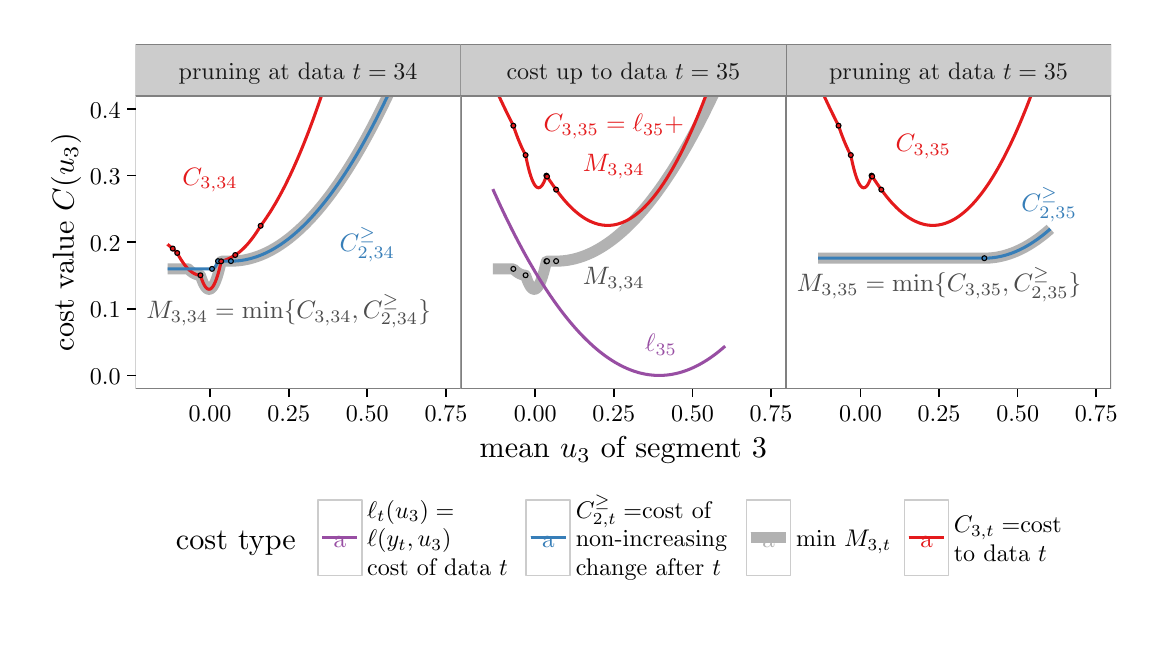
\begin{tikzpicture}[x=1pt,y=1pt]
\definecolor{fillColor}{RGB}{255,255,255}
\path[use as bounding box,fill=fillColor,fill opacity=0.00] (0,0) rectangle (397.48,216.81);
\begin{scope}
\path[clip] (  0.00,  0.00) rectangle (397.48,216.81);
\definecolor{drawColor}{RGB}{255,255,255}
\definecolor{fillColor}{RGB}{255,255,255}

\path[draw=drawColor,line width= 0.6pt,line join=round,line cap=round,fill=fillColor] (  0.00,  0.00) rectangle (397.48,216.81);
\end{scope}
\begin{scope}
\path[clip] ( 38.97,192.23) rectangle (156.48,210.81);
\definecolor{drawColor}{gray}{0.50}
\definecolor{fillColor}{gray}{0.80}

\path[draw=drawColor,line width= 0.2pt,line join=round,line cap=round,fill=fillColor] ( 38.97,192.23) rectangle (156.48,210.81);
\definecolor{drawColor}{gray}{0.10}

\node[text=drawColor,anchor=base,inner sep=0pt, outer sep=0pt, scale=  0.87] at ( 97.72,198.23) {pruning at data $t=34$};
\end{scope}
\begin{scope}
\path[clip] (156.48,192.23) rectangle (273.98,210.81);
\definecolor{drawColor}{gray}{0.50}
\definecolor{fillColor}{gray}{0.80}

\path[draw=drawColor,line width= 0.2pt,line join=round,line cap=round,fill=fillColor] (156.48,192.23) rectangle (273.98,210.81);
\definecolor{drawColor}{gray}{0.10}

\node[text=drawColor,anchor=base,inner sep=0pt, outer sep=0pt, scale=  0.87] at (215.23,198.23) {cost up to data $t=35$};
\end{scope}
\begin{scope}
\path[clip] (273.98,192.23) rectangle (391.48,210.81);
\definecolor{drawColor}{gray}{0.50}
\definecolor{fillColor}{gray}{0.80}

\path[draw=drawColor,line width= 0.2pt,line join=round,line cap=round,fill=fillColor] (273.98,192.23) rectangle (391.48,210.81);
\definecolor{drawColor}{gray}{0.10}

\node[text=drawColor,anchor=base,inner sep=0pt, outer sep=0pt, scale=  0.87] at (332.73,198.23) {pruning at data $t=35$};
\end{scope}
\begin{scope}
\path[clip] ( 38.97, 86.33) rectangle (156.48,192.23);
\definecolor{fillColor}{RGB}{255,255,255}

\path[fill=fillColor] ( 38.97, 86.33) rectangle (156.48,192.23);
\definecolor{drawColor}{gray}{0.70}

\path[draw=drawColor,line width= 4.0pt,line join=round] ( 50.58,129.65) --
	( 50.65,129.65) --
	( 50.73,129.65) --
	( 50.80,129.65) --
	( 50.88,129.65) --
	( 50.95,129.65) --
	( 51.02,129.65) --
	( 51.10,129.65) --
	( 51.17,129.65) --
	( 51.25,129.65) --
	( 51.32,129.65) --
	( 51.40,129.65) --
	( 51.47,129.65) --
	( 51.55,129.65) --
	( 51.62,129.65) --
	( 51.70,129.65) --
	( 51.77,129.65) --
	( 51.85,129.65) --
	( 51.92,129.65) --
	( 52.00,129.65) --
	( 52.07,129.65) --
	( 52.15,129.65) --
	( 52.22,129.65) --
	( 52.30,129.65) --
	( 52.37,129.65) --
	( 52.45,129.65) --
	( 52.52,129.65) --
	( 52.60,129.65) --
	( 52.67,129.65) --
	( 52.75,129.65) --
	( 52.82,129.65) --
	( 52.90,129.65) --
	( 52.97,129.65) --
	( 53.05,129.65) --
	( 53.12,129.65) --
	( 53.20,129.65) --
	( 53.27,129.65) --
	( 53.35,129.65) --
	( 53.42,129.65) --
	( 53.50,129.65) --
	( 53.57,129.65) --
	( 53.65,129.65) --
	( 53.72,129.65) --
	( 53.80,129.65) --
	( 53.87,129.65) --
	( 53.95,129.65) --
	( 54.02,129.65) --
	( 54.10,129.65) --
	( 54.17,129.65) --
	( 54.25,129.65) --
	( 54.32,129.65) --
	( 54.39,129.65) --
	( 54.47,129.65) --
	( 54.54,129.65) --
	( 54.62,129.65) --
	( 54.69,129.65) --
	( 54.77,129.65) --
	( 54.84,129.65) --
	( 54.92,129.65) --
	( 54.99,129.65) --
	( 55.07,129.65) --
	( 55.14,129.65) --
	( 55.22,129.65) --
	( 55.29,129.65) --
	( 55.37,129.65) --
	( 55.44,129.65) --
	( 55.52,129.65) --
	( 55.59,129.65) --
	( 55.67,129.65) --
	( 55.74,129.65) --
	( 55.82,129.65) --
	( 55.89,129.65) --
	( 55.97,129.65) --
	( 56.04,129.65) --
	( 56.12,129.65) --
	( 56.19,129.65) --
	( 56.27,129.65) --
	( 56.34,129.65) --
	( 56.42,129.65) --
	( 56.49,129.65) --
	( 56.57,129.65) --
	( 56.64,129.65) --
	( 56.72,129.65) --
	( 56.79,129.65) --
	( 56.87,129.65) --
	( 56.94,129.65) --
	( 57.02,129.65) --
	( 57.09,129.65) --
	( 57.17,129.65) --
	( 57.24,129.65) --
	( 57.32,129.65) --
	( 57.39,129.65) --
	( 57.47,129.65) --
	( 57.54,129.65) --
	( 57.61,129.65) --
	( 57.69,129.65) --
	( 57.76,129.65) --
	( 57.84,129.65) --
	( 57.91,129.65) --
	( 57.99,129.65) --
	( 57.99,129.65) --
	( 58.03,129.60) --
	( 58.08,129.56) --
	( 58.12,129.51) --
	( 58.17,129.47) --
	( 58.21,129.43) --
	( 58.26,129.38) --
	( 58.30,129.34) --
	( 58.35,129.30) --
	( 58.39,129.26) --
	( 58.44,129.21) --
	( 58.48,129.17) --
	( 58.53,129.13) --
	( 58.57,129.09) --
	( 58.62,129.05) --
	( 58.66,129.02) --
	( 58.71,128.98) --
	( 58.75,128.94) --
	( 58.79,128.90) --
	( 58.84,128.86) --
	( 58.88,128.83) --
	( 58.93,128.79) --
	( 58.97,128.76) --
	( 59.02,128.72) --
	( 59.06,128.69) --
	( 59.11,128.65) --
	( 59.15,128.62) --
	( 59.20,128.58) --
	( 59.24,128.55) --
	( 59.29,128.52) --
	( 59.33,128.49) --
	( 59.38,128.45) --
	( 59.42,128.42) --
	( 59.47,128.39) --
	( 59.51,128.36) --
	( 59.55,128.33) --
	( 59.60,128.30) --
	( 59.64,128.27) --
	( 59.69,128.24) --
	( 59.73,128.22) --
	( 59.78,128.19) --
	( 59.82,128.16) --
	( 59.87,128.13) --
	( 59.91,128.11) --
	( 59.96,128.08) --
	( 60.00,128.06) --
	( 60.05,128.03) --
	( 60.09,128.01) --
	( 60.14,127.98) --
	( 60.18,127.96) --
	( 60.23,127.94) --
	( 60.27,127.91) --
	( 60.32,127.89) --
	( 60.36,127.87) --
	( 60.40,127.85) --
	( 60.45,127.83) --
	( 60.49,127.81) --
	( 60.54,127.79) --
	( 60.58,127.77) --
	( 60.63,127.75) --
	( 60.67,127.73) --
	( 60.72,127.71) --
	( 60.76,127.69) --
	( 60.81,127.67) --
	( 60.85,127.66) --
	( 60.90,127.64) --
	( 60.94,127.62) --
	( 60.99,127.61) --
	( 61.03,127.59) --
	( 61.08,127.58) --
	( 61.12,127.57) --
	( 61.17,127.55) --
	( 61.21,127.54) --
	( 61.25,127.52) --
	( 61.30,127.51) --
	( 61.34,127.50) --
	( 61.39,127.49) --
	( 61.43,127.48) --
	( 61.48,127.47) --
	( 61.52,127.46) --
	( 61.57,127.45) --
	( 61.61,127.44) --
	( 61.66,127.43) --
	( 61.70,127.42) --
	( 61.75,127.41) --
	( 61.79,127.40) --
	( 61.84,127.40) --
	( 61.88,127.39) --
	( 61.93,127.38) --
	( 61.97,127.38) --
	( 62.02,127.37) --
	( 62.06,127.37) --
	( 62.10,127.36) --
	( 62.15,127.36) --
	( 62.19,127.36) --
	( 62.24,127.35) --
	( 62.28,127.35) --
	( 62.33,127.35) --
	( 62.37,127.35) --
	( 62.42,127.35) --
	( 62.42,127.35) --
	( 62.49,127.10) --
	( 62.57,126.86) --
	( 62.65,126.63) --
	( 62.72,126.41) --
	( 62.80,126.19) --
	( 62.87,125.97) --
	( 62.95,125.77) --
	( 63.03,125.56) --
	( 63.10,125.37) --
	( 63.18,125.18) --
	( 63.25,125.00) --
	( 63.33,124.82) --
	( 63.40,124.65) --
	( 63.48,124.48) --
	( 63.56,124.32) --
	( 63.63,124.17) --
	( 63.71,124.02) --
	( 63.78,123.88) --
	( 63.86,123.74) --
	( 63.94,123.61) --
	( 64.01,123.49) --
	( 64.09,123.37) --
	( 64.16,123.26) --
	( 64.24,123.16) --
	( 64.32,123.06) --
	( 64.39,122.96) --
	( 64.47,122.88) --
	( 64.54,122.80) --
	( 64.62,122.72) --
	( 64.69,122.65) --
	( 64.77,122.59) --
	( 64.85,122.53) --
	( 64.92,122.48) --
	( 65.00,122.43) --
	( 65.07,122.39) --
	( 65.15,122.36) --
	( 65.23,122.33) --
	( 65.30,122.31) --
	( 65.38,122.30) --
	( 65.45,122.29) --
	( 65.53,122.28) --
	( 65.61,122.29) --
	( 65.68,122.30) --
	( 65.76,122.31) --
	( 65.83,122.33) --
	( 65.91,122.36) --
	( 65.98,122.39) --
	( 66.06,122.43) --
	( 66.14,122.48) --
	( 66.21,122.53) --
	( 66.29,122.58) --
	( 66.36,122.65) --
	( 66.44,122.71) --
	( 66.52,122.79) --
	( 66.59,122.87) --
	( 66.67,122.96) --
	( 66.74,123.05) --
	( 66.82,123.15) --
	( 66.90,123.25) --
	( 66.97,123.37) --
	( 67.05,123.48) --
	( 67.12,123.61) --
	( 67.20,123.73) --
	( 67.28,123.87) --
	( 67.35,124.01) --
	( 67.43,124.16) --
	( 67.50,124.31) --
	( 67.58,124.47) --
	( 67.65,124.64) --
	( 67.73,124.81) --
	( 67.81,124.98) --
	( 67.88,125.17) --
	( 67.96,125.36) --
	( 68.03,125.55) --
	( 68.11,125.75) --
	( 68.19,125.96) --
	( 68.26,126.17) --
	( 68.34,126.39) --
	( 68.41,126.62) --
	( 68.49,126.85) --
	( 68.57,127.09) --
	( 68.64,127.33) --
	( 68.72,127.58) --
	( 68.79,127.83) --
	( 68.87,128.09) --
	( 68.94,128.36) --
	( 69.02,128.63) --
	( 69.10,128.91) --
	( 69.17,129.20) --
	( 69.25,129.49) --
	( 69.32,129.79) --
	( 69.40,130.09) --
	( 69.48,130.40) --
	( 69.55,130.72) --
	( 69.63,131.04) --
	( 69.70,131.36) --
	( 69.78,131.70) --
	( 69.86,132.04) --
	( 69.93,132.38) --
	( 69.93,132.38) --
	( 69.93,132.38) --
	( 69.94,132.38) --
	( 69.94,132.38) --
	( 69.94,132.39) --
	( 69.94,132.39) --
	( 69.95,132.39) --
	( 69.95,132.39) --
	( 69.95,132.39) --
	( 69.95,132.39) --
	( 69.96,132.39) --
	( 69.96,132.39) --
	( 69.96,132.39) --
	( 69.96,132.39) --
	( 69.96,132.39) --
	( 69.97,132.39) --
	( 69.97,132.39) --
	( 69.97,132.39) --
	( 69.97,132.39) --
	( 69.98,132.39) --
	( 69.98,132.40) --
	( 69.98,132.40) --
	( 69.98,132.40) --
	( 69.99,132.40) --
	( 69.99,132.40) --
	( 69.99,132.40) --
	( 69.99,132.40) --
	( 70.00,132.40) --
	( 70.00,132.40) --
	( 70.00,132.40) --
	( 70.00,132.40) --
	( 70.01,132.40) --
	( 70.01,132.40) --
	( 70.01,132.40) --
	( 70.01,132.40) --
	( 70.02,132.40) --
	( 70.02,132.41) --
	( 70.02,132.41) --
	( 70.02,132.41) --
	( 70.02,132.41) --
	( 70.03,132.41) --
	( 70.03,132.41) --
	( 70.03,132.41) --
	( 70.03,132.41) --
	( 70.04,132.41) --
	( 70.04,132.41) --
	( 70.04,132.41) --
	( 70.04,132.41) --
	( 70.05,132.41) --
	( 70.05,132.41) --
	( 70.05,132.41) --
	( 70.05,132.42) --
	( 70.06,132.42) --
	( 70.06,132.42) --
	( 70.06,132.42) --
	( 70.06,132.42) --
	( 70.07,132.42) --
	( 70.07,132.42) --
	( 70.07,132.42) --
	( 70.07,132.42) --
	( 70.08,132.42) --
	( 70.08,132.42) --
	( 70.08,132.42) --
	( 70.08,132.42) --
	( 70.08,132.42) --
	( 70.09,132.42) --
	( 70.09,132.42) --
	( 70.09,132.43) --
	( 70.09,132.43) --
	( 70.10,132.43) --
	( 70.10,132.43) --
	( 70.10,132.43) --
	( 70.10,132.43) --
	( 70.11,132.43) --
	( 70.11,132.43) --
	( 70.11,132.43) --
	( 70.11,132.43) --
	( 70.12,132.43) --
	( 70.12,132.43) --
	( 70.12,132.43) --
	( 70.12,132.43) --
	( 70.13,132.43) --
	( 70.13,132.44) --
	( 70.13,132.44) --
	( 70.13,132.44) --
	( 70.14,132.44) --
	( 70.14,132.44) --
	( 70.14,132.44) --
	( 70.14,132.44) --
	( 70.14,132.44) --
	( 70.15,132.44) --
	( 70.15,132.44) --
	( 70.15,132.44) --
	( 70.15,132.44) --
	( 70.16,132.44) --
	( 70.16,132.44) --
	( 70.16,132.44) --
	( 70.16,132.45) --
	( 70.17,132.45) --
	( 70.17,132.45) --
	( 70.17,132.45) --
	( 70.20,132.45) --
	( 70.24,132.45) --
	( 70.27,132.45) --
	( 70.30,132.45) --
	( 70.33,132.45) --
	( 70.37,132.45) --
	( 70.40,132.45) --
	( 70.43,132.45) --
	( 70.47,132.45) --
	( 70.50,132.45) --
	( 70.53,132.45) --
	( 70.57,132.45) --
	( 70.60,132.45) --
	( 70.63,132.45) --
	( 70.67,132.45) --
	( 70.70,132.45) --
	( 70.73,132.45) --
	( 70.77,132.45) --
	( 70.80,132.45) --
	( 70.83,132.45) --
	( 70.87,132.45) --
	( 70.90,132.45) --
	( 70.93,132.45) --
	( 70.96,132.45) --
	( 71.00,132.45) --
	( 71.03,132.45) --
	( 71.06,132.45) --
	( 71.10,132.45) --
	( 71.13,132.45) --
	( 71.16,132.45) --
	( 71.20,132.45) --
	( 71.23,132.45) --
	( 71.26,132.45) --
	( 71.30,132.45) --
	( 71.33,132.45) --
	( 71.36,132.45) --
	( 71.40,132.45) --
	( 71.43,132.45) --
	( 71.46,132.45) --
	( 71.50,132.45) --
	( 71.53,132.45) --
	( 71.56,132.45) --
	( 71.59,132.45) --
	( 71.63,132.45) --
	( 71.66,132.45) --
	( 71.69,132.45) --
	( 71.73,132.45) --
	( 71.76,132.45) --
	( 71.79,132.45) --
	( 71.83,132.45) --
	( 71.86,132.45) --
	( 71.89,132.45) --
	( 71.93,132.45) --
	( 71.96,132.45) --
	( 71.99,132.45) --
	( 72.03,132.45) --
	( 72.06,132.45) --
	( 72.09,132.45) --
	( 72.13,132.45) --
	( 72.16,132.45) --
	( 72.19,132.45) --
	( 72.23,132.45) --
	( 72.26,132.45) --
	( 72.29,132.45) --
	( 72.32,132.45) --
	( 72.36,132.45) --
	( 72.39,132.45) --
	( 72.42,132.45) --
	( 72.46,132.45) --
	( 72.49,132.45) --
	( 72.52,132.45) --
	( 72.56,132.45) --
	( 72.59,132.45) --
	( 72.62,132.45) --
	( 72.66,132.45) --
	( 72.69,132.45) --
	( 72.72,132.45) --
	( 72.76,132.45) --
	( 72.79,132.45) --
	( 72.82,132.45) --
	( 72.86,132.45) --
	( 72.89,132.45) --
	( 72.92,132.45) --
	( 72.95,132.45) --
	( 72.99,132.45) --
	( 73.02,132.45) --
	( 73.05,132.45) --
	( 73.09,132.45) --
	( 73.12,132.45) --
	( 73.15,132.45) --
	( 73.19,132.45) --
	( 73.22,132.45) --
	( 73.25,132.45) --
	( 73.29,132.45) --
	( 73.32,132.45) --
	( 73.35,132.45) --
	( 73.39,132.45) --
	( 73.42,132.45) --
	( 73.45,132.45) --
	( 73.45,132.45) --
	( 74.07,132.45) --
	( 74.69,132.47) --
	( 75.30,132.51) --
	( 75.92,132.56) --
	( 76.54,132.62) --
	( 77.15,132.70) --
	( 77.77,132.79) --
	( 78.39,132.90) --
	( 79.00,133.02) --
	( 79.62,133.16) --
	( 80.24,133.30) --
	( 80.85,133.47) --
	( 81.47,133.65) --
	( 82.09,133.84) --
	( 82.71,134.04) --
	( 83.32,134.26) --
	( 83.94,134.50) --
	( 84.56,134.74) --
	( 85.17,135.01) --
	( 85.79,135.28) --
	( 86.41,135.57) --
	( 87.02,135.88) --
	( 87.64,136.20) --
	( 88.26,136.53) --
	( 88.87,136.88) --
	( 89.49,137.24) --
	( 90.11,137.62) --
	( 90.73,138.01) --
	( 91.34,138.41) --
	( 91.96,138.83) --
	( 92.58,139.26) --
	( 93.19,139.71) --
	( 93.81,140.17) --
	( 94.43,140.64) --
	( 95.04,141.13) --
	( 95.66,141.64) --
	( 96.28,142.16) --
	( 96.89,142.69) --
	( 97.51,143.23) --
	( 98.13,143.79) --
	( 98.74,144.37) --
	( 99.36,144.96) --
	( 99.98,145.56) --
	(100.60,146.18) --
	(101.21,146.81) --
	(101.83,147.45) --
	(102.45,148.11) --
	(103.06,148.79) --
	(103.68,149.47) --
	(104.30,150.18) --
	(104.91,150.89) --
	(105.53,151.62) --
	(106.15,152.37) --
	(106.76,153.13) --
	(107.38,153.90) --
	(108.00,154.69) --
	(108.62,155.49) --
	(109.23,156.30) --
	(109.85,157.13) --
	(110.47,157.98) --
	(111.08,158.84) --
	(111.70,159.71) --
	(112.32,160.59) --
	(112.93,161.50) --
	(113.55,162.41) --
	(114.17,163.34) --
	(114.78,164.28) --
	(115.40,165.24) --
	(116.02,166.21) --
	(116.63,167.20) --
	(117.25,168.20) --
	(117.87,169.21) --
	(118.49,170.24) --
	(119.10,171.28) --
	(119.72,172.34) --
	(120.34,173.41) --
	(120.95,174.49) --
	(121.57,175.59) --
	(122.19,176.71) --
	(122.80,177.84) --
	(123.42,178.98) --
	(124.04,180.13) --
	(124.65,181.30) --
	(125.27,182.49) --
	(125.89,183.69) --
	(126.50,184.90) --
	(127.12,186.13) --
	(127.74,187.37) --
	(128.36,188.62) --
	(128.97,189.89) --
	(129.59,191.18) --
	(130.21,192.47) --
	(130.82,193.79) --
	(131.44,195.11) --
	(132.06,196.45) --
	(132.67,197.81) --
	(133.29,199.17) --
	(133.91,200.56) --
	(134.52,201.95);
\definecolor{drawColor}{RGB}{228,26,28}

\path[draw=drawColor,line width= 1.1pt,line join=round] ( 50.58,138.50) --
	( 50.59,138.48) --
	( 50.61,138.47) --
	( 50.63,138.45) --
	( 50.65,138.44) --
	( 50.67,138.42) --
	( 50.69,138.41) --
	( 50.71,138.39) --
	( 50.73,138.37) --
	( 50.74,138.36) --
	( 50.76,138.34) --
	( 50.78,138.33) --
	( 50.80,138.31) --
	( 50.82,138.29) --
	( 50.84,138.28) --
	( 50.86,138.26) --
	( 50.88,138.25) --
	( 50.89,138.23) --
	( 50.91,138.21) --
	( 50.93,138.20) --
	( 50.95,138.18) --
	( 50.97,138.17) --
	( 50.99,138.15) --
	( 51.01,138.14) --
	( 51.03,138.12) --
	( 51.04,138.10) --
	( 51.06,138.09) --
	( 51.08,138.07) --
	( 51.10,138.06) --
	( 51.12,138.04) --
	( 51.14,138.03) --
	( 51.16,138.01) --
	( 51.18,138.00) --
	( 51.20,137.98) --
	( 51.21,137.96) --
	( 51.23,137.95) --
	( 51.25,137.93) --
	( 51.27,137.92) --
	( 51.29,137.90) --
	( 51.31,137.89) --
	( 51.33,137.87) --
	( 51.35,137.86) --
	( 51.36,137.84) --
	( 51.38,137.82) --
	( 51.40,137.81) --
	( 51.42,137.79) --
	( 51.44,137.78) --
	( 51.46,137.76) --
	( 51.48,137.75) --
	( 51.50,137.73) --
	( 51.51,137.72) --
	( 51.53,137.70) --
	( 51.55,137.69) --
	( 51.57,137.67) --
	( 51.59,137.66) --
	( 51.61,137.64) --
	( 51.63,137.63) --
	( 51.65,137.61) --
	( 51.66,137.59) --
	( 51.68,137.58) --
	( 51.70,137.56) --
	( 51.72,137.55) --
	( 51.74,137.53) --
	( 51.76,137.52) --
	( 51.78,137.50) --
	( 51.80,137.49) --
	( 51.81,137.47) --
	( 51.83,137.46) --
	( 51.85,137.44) --
	( 51.87,137.43) --
	( 51.89,137.41) --
	( 51.91,137.40) --
	( 51.93,137.38) --
	( 51.95,137.37) --
	( 51.96,137.35) --
	( 51.98,137.34) --
	( 52.00,137.32) --
	( 52.02,137.31) --
	( 52.04,137.29) --
	( 52.06,137.28) --
	( 52.08,137.26) --
	( 52.10,137.25) --
	( 52.12,137.23) --
	( 52.13,137.22) --
	( 52.15,137.20) --
	( 52.17,137.19) --
	( 52.19,137.17) --
	( 52.21,137.16) --
	( 52.23,137.14) --
	( 52.25,137.13) --
	( 52.27,137.11) --
	( 52.28,137.10) --
	( 52.30,137.08) --
	( 52.32,137.07) --
	( 52.34,137.05) --
	( 52.36,137.04) --
	( 52.38,137.02) --
	( 52.40,137.01) --
	( 52.42,137.00) --
	( 52.43,136.98) --
	( 52.43,136.98) --
	( 52.45,136.96) --
	( 52.47,136.95) --
	( 52.48,136.93) --
	( 52.50,136.91) --
	( 52.52,136.90) --
	( 52.53,136.88) --
	( 52.55,136.86) --
	( 52.56,136.85) --
	( 52.58,136.83) --
	( 52.60,136.81) --
	( 52.61,136.80) --
	( 52.63,136.78) --
	( 52.65,136.76) --
	( 52.66,136.74) --
	( 52.68,136.73) --
	( 52.69,136.71) --
	( 52.71,136.69) --
	( 52.73,136.68) --
	( 52.74,136.66) --
	( 52.76,136.65) --
	( 52.78,136.63) --
	( 52.79,136.61) --
	( 52.81,136.60) --
	( 52.82,136.58) --
	( 52.84,136.56) --
	( 52.86,136.55) --
	( 52.87,136.53) --
	( 52.89,136.51) --
	( 52.90,136.50) --
	( 52.92,136.48) --
	( 52.94,136.46) --
	( 52.95,136.45) --
	( 52.97,136.43) --
	( 52.99,136.41) --
	( 53.00,136.40) --
	( 53.02,136.38) --
	( 53.03,136.37) --
	( 53.05,136.35) --
	( 53.07,136.33) --
	( 53.08,136.32) --
	( 53.10,136.30) --
	( 53.12,136.28) --
	( 53.13,136.27) --
	( 53.15,136.25) --
	( 53.16,136.24) --
	( 53.18,136.22) --
	( 53.20,136.20) --
	( 53.21,136.19) --
	( 53.23,136.17) --
	( 53.25,136.16) --
	( 53.26,136.14) --
	( 53.28,136.12) --
	( 53.29,136.11) --
	( 53.31,136.09) --
	( 53.33,136.08) --
	( 53.34,136.06) --
	( 53.36,136.04) --
	( 53.38,136.03) --
	( 53.39,136.01) --
	( 53.41,136.00) --
	( 53.42,135.98) --
	( 53.44,135.97) --
	( 53.46,135.95) --
	( 53.47,135.93) --
	( 53.49,135.92) --
	( 53.51,135.90) --
	( 53.52,135.89) --
	( 53.54,135.87) --
	( 53.55,135.86) --
	( 53.57,135.84) --
	( 53.59,135.82) --
	( 53.60,135.81) --
	( 53.62,135.79) --
	( 53.64,135.78) --
	( 53.65,135.76) --
	( 53.67,135.75) --
	( 53.68,135.73) --
	( 53.70,135.72) --
	( 53.72,135.70) --
	( 53.73,135.69) --
	( 53.75,135.67) --
	( 53.77,135.65) --
	( 53.78,135.64) --
	( 53.80,135.62) --
	( 53.81,135.61) --
	( 53.83,135.59) --
	( 53.85,135.58) --
	( 53.86,135.56) --
	( 53.88,135.55) --
	( 53.90,135.53) --
	( 53.91,135.52) --
	( 53.93,135.50) --
	( 53.94,135.49) --
	( 53.96,135.47) --
	( 53.98,135.46) --
	( 53.99,135.44) --
	( 54.01,135.43) --
	( 54.02,135.41) --
	( 54.04,135.40) --
	( 54.04,135.40) --
	( 54.13,135.24) --
	( 54.21,135.08) --
	( 54.30,134.92) --
	( 54.38,134.77) --
	( 54.46,134.61) --
	( 54.55,134.46) --
	( 54.63,134.31) --
	( 54.72,134.16) --
	( 54.80,134.02) --
	( 54.89,133.87) --
	( 54.97,133.73) --
	( 55.06,133.58) --
	( 55.14,133.44) --
	( 55.23,133.31) --
	( 55.31,133.17) --
	( 55.39,133.03) --
	( 55.48,132.90) --
	( 55.56,132.77) --
	( 55.65,132.63) --
	( 55.73,132.50) --
	( 55.82,132.38) --
	( 55.90,132.25) --
	( 55.99,132.13) --
	( 56.07,132.00) --
	( 56.16,131.88) --
	( 56.24,131.76) --
	( 56.33,131.64) --
	( 56.41,131.53) --
	( 56.49,131.41) --
	( 56.58,131.30) --
	( 56.66,131.19) --
	( 56.75,131.08) --
	( 56.83,130.97) --
	( 56.92,130.86) --
	( 57.00,130.76) --
	( 57.09,130.65) --
	( 57.17,130.55) --
	( 57.26,130.45) --
	( 57.34,130.35) --
	( 57.43,130.25) --
	( 57.51,130.16) --
	( 57.59,130.06) --
	( 57.68,129.97) --
	( 57.76,129.88) --
	( 57.85,129.79) --
	( 57.93,129.70) --
	( 58.02,129.62) --
	( 58.10,129.53) --
	( 58.19,129.45) --
	( 58.27,129.37) --
	( 58.36,129.29) --
	( 58.44,129.21) --
	( 58.53,129.13) --
	( 58.61,129.06) --
	( 58.69,128.99) --
	( 58.78,128.91) --
	( 58.86,128.84) --
	( 58.95,128.78) --
	( 59.03,128.71) --
	( 59.12,128.64) --
	( 59.20,128.58) --
	( 59.29,128.52) --
	( 59.37,128.46) --
	( 59.46,128.40) --
	( 59.54,128.34) --
	( 59.63,128.29) --
	( 59.71,128.23) --
	( 59.79,128.18) --
	( 59.88,128.13) --
	( 59.96,128.08) --
	( 60.05,128.03) --
	( 60.13,127.98) --
	( 60.22,127.94) --
	( 60.30,127.90) --
	( 60.39,127.86) --
	( 60.47,127.82) --
	( 60.56,127.78) --
	( 60.64,127.74) --
	( 60.73,127.71) --
	( 60.81,127.67) --
	( 60.89,127.64) --
	( 60.98,127.61) --
	( 61.06,127.58) --
	( 61.15,127.56) --
	( 61.23,127.53) --
	( 61.32,127.51) --
	( 61.40,127.49) --
	( 61.49,127.46) --
	( 61.57,127.45) --
	( 61.66,127.43) --
	( 61.74,127.41) --
	( 61.83,127.40) --
	( 61.91,127.39) --
	( 61.99,127.38) --
	( 62.08,127.37) --
	( 62.16,127.36) --
	( 62.25,127.35) --
	( 62.33,127.35) --
	( 62.42,127.35) --
	( 62.42,127.35) --
	( 62.49,127.10) --
	( 62.57,126.86) --
	( 62.65,126.63) --
	( 62.72,126.41) --
	( 62.80,126.19) --
	( 62.87,125.97) --
	( 62.95,125.77) --
	( 63.03,125.56) --
	( 63.10,125.37) --
	( 63.18,125.18) --
	( 63.25,125.00) --
	( 63.33,124.82) --
	( 63.40,124.65) --
	( 63.48,124.48) --
	( 63.56,124.32) --
	( 63.63,124.17) --
	( 63.71,124.02) --
	( 63.78,123.88) --
	( 63.86,123.74) --
	( 63.94,123.61) --
	( 64.01,123.49) --
	( 64.09,123.37) --
	( 64.16,123.26) --
	( 64.24,123.16) --
	( 64.32,123.06) --
	( 64.39,122.96) --
	( 64.47,122.88) --
	( 64.54,122.80) --
	( 64.62,122.72) --
	( 64.69,122.65) --
	( 64.77,122.59) --
	( 64.85,122.53) --
	( 64.92,122.48) --
	( 65.00,122.43) --
	( 65.07,122.39) --
	( 65.15,122.36) --
	( 65.23,122.33) --
	( 65.30,122.31) --
	( 65.38,122.30) --
	( 65.45,122.29) --
	( 65.53,122.28) --
	( 65.61,122.29) --
	( 65.68,122.30) --
	( 65.76,122.31) --
	( 65.83,122.33) --
	( 65.91,122.36) --
	( 65.98,122.39) --
	( 66.06,122.43) --
	( 66.14,122.48) --
	( 66.21,122.53) --
	( 66.29,122.58) --
	( 66.36,122.65) --
	( 66.44,122.71) --
	( 66.52,122.79) --
	( 66.59,122.87) --
	( 66.67,122.96) --
	( 66.74,123.05) --
	( 66.82,123.15) --
	( 66.90,123.25) --
	( 66.97,123.37) --
	( 67.05,123.48) --
	( 67.12,123.61) --
	( 67.20,123.73) --
	( 67.28,123.87) --
	( 67.35,124.01) --
	( 67.43,124.16) --
	( 67.50,124.31) --
	( 67.58,124.47) --
	( 67.65,124.64) --
	( 67.73,124.81) --
	( 67.81,124.98) --
	( 67.88,125.17) --
	( 67.96,125.36) --
	( 68.03,125.55) --
	( 68.11,125.75) --
	( 68.19,125.96) --
	( 68.26,126.17) --
	( 68.34,126.39) --
	( 68.41,126.62) --
	( 68.49,126.85) --
	( 68.57,127.09) --
	( 68.64,127.33) --
	( 68.72,127.58) --
	( 68.79,127.83) --
	( 68.87,128.09) --
	( 68.94,128.36) --
	( 69.02,128.63) --
	( 69.10,128.91) --
	( 69.17,129.20) --
	( 69.25,129.49) --
	( 69.32,129.79) --
	( 69.40,130.09) --
	( 69.48,130.40) --
	( 69.55,130.72) --
	( 69.63,131.04) --
	( 69.70,131.36) --
	( 69.78,131.70) --
	( 69.86,132.04) --
	( 69.93,132.38) --
	( 69.93,132.38) --
	( 69.98,132.40) --
	( 70.03,132.41) --
	( 70.09,132.42) --
	( 70.14,132.44) --
	( 70.19,132.45) --
	( 70.24,132.47) --
	( 70.29,132.48) --
	( 70.34,132.50) --
	( 70.39,132.51) --
	( 70.44,132.53) --
	( 70.49,132.54) --
	( 70.55,132.56) --
	( 70.60,132.57) --
	( 70.65,132.59) --
	( 70.70,132.60) --
	( 70.75,132.62) --
	( 70.80,132.64) --
	( 70.85,132.65) --
	( 70.90,132.67) --
	( 70.96,132.69) --
	( 71.01,132.70) --
	( 71.06,132.72) --
	( 71.11,132.74) --
	( 71.16,132.76) --
	( 71.21,132.78) --
	( 71.26,132.79) --
	( 71.31,132.81) --
	( 71.37,132.83) --
	( 71.42,132.85) --
	( 71.47,132.87) --
	( 71.52,132.89) --
	( 71.57,132.91) --
	( 71.62,132.93) --
	( 71.67,132.95) --
	( 71.72,132.97) --
	( 71.78,132.99) --
	( 71.83,133.01) --
	( 71.88,133.03) --
	( 71.93,133.05) --
	( 71.98,133.07) --
	( 72.03,133.09) --
	( 72.08,133.11) --
	( 72.13,133.13) --
	( 72.19,133.16) --
	( 72.24,133.18) --
	( 72.29,133.20) --
	( 72.34,133.22) --
	( 72.39,133.24) --
	( 72.44,133.27) --
	( 72.49,133.29) --
	( 72.54,133.31) --
	( 72.60,133.34) --
	( 72.65,133.36) --
	( 72.70,133.38) --
	( 72.75,133.41) --
	( 72.80,133.43) --
	( 72.85,133.46) --
	( 72.90,133.48) --
	( 72.95,133.51) --
	( 73.01,133.53) --
	( 73.06,133.56) --
	( 73.11,133.58) --
	( 73.16,133.61) --
	( 73.21,133.63) --
	( 73.26,133.66) --
	( 73.31,133.68) --
	( 73.36,133.71) --
	( 73.42,133.74) --
	( 73.47,133.76) --
	( 73.52,133.79) --
	( 73.57,133.82) --
	( 73.62,133.84) --
	( 73.67,133.87) --
	( 73.72,133.90) --
	( 73.77,133.93) --
	( 73.83,133.96) --
	( 73.88,133.98) --
	( 73.93,134.01) --
	( 73.98,134.04) --
	( 74.03,134.07) --
	( 74.08,134.10) --
	( 74.13,134.13) --
	( 74.18,134.16) --
	( 74.24,134.19) --
	( 74.29,134.22) --
	( 74.34,134.25) --
	( 74.39,134.28) --
	( 74.44,134.31) --
	( 74.49,134.34) --
	( 74.54,134.37) --
	( 74.59,134.40) --
	( 74.65,134.43) --
	( 74.70,134.46) --
	( 74.75,134.49) --
	( 74.80,134.53) --
	( 74.85,134.56) --
	( 74.90,134.59) --
	( 74.95,134.62) --
	( 75.00,134.65) --
	( 75.00,134.65) --
	( 75.10,134.71) --
	( 75.19,134.77) --
	( 75.28,134.84) --
	( 75.38,134.90) --
	( 75.47,134.96) --
	( 75.56,135.03) --
	( 75.65,135.09) --
	( 75.75,135.16) --
	( 75.84,135.22) --
	( 75.93,135.29) --
	( 76.02,135.36) --
	( 76.12,135.43) --
	( 76.21,135.50) --
	( 76.30,135.57) --
	( 76.40,135.65) --
	( 76.49,135.72) --
	( 76.58,135.80) --
	( 76.67,135.87) --
	( 76.77,135.95) --
	( 76.86,136.03) --
	( 76.95,136.11) --
	( 77.04,136.19) --
	( 77.14,136.27) --
	( 77.23,136.35) --
	( 77.32,136.43) --
	( 77.41,136.51) --
	( 77.51,136.60) --
	( 77.60,136.68) --
	( 77.69,136.77) --
	( 77.79,136.86) --
	( 77.88,136.95) --
	( 77.97,137.04) --
	( 78.06,137.13) --
	( 78.16,137.22) --
	( 78.25,137.31) --
	( 78.34,137.40) --
	( 78.43,137.50) --
	( 78.53,137.59) --
	( 78.62,137.69) --
	( 78.71,137.78) --
	( 78.81,137.88) --
	( 78.90,137.98) --
	( 78.99,138.08) --
	( 79.08,138.18) --
	( 79.18,138.28) --
	( 79.27,138.39) --
	( 79.36,138.49) --
	( 79.45,138.59) --
	( 79.55,138.70) --
	( 79.64,138.81) --
	( 79.73,138.91) --
	( 79.83,139.02) --
	( 79.92,139.13) --
	( 80.01,139.24) --
	( 80.10,139.35) --
	( 80.20,139.47) --
	( 80.29,139.58) --
	( 80.38,139.69) --
	( 80.47,139.81) --
	( 80.57,139.93) --
	( 80.66,140.04) --
	( 80.75,140.16) --
	( 80.84,140.28) --
	( 80.94,140.40) --
	( 81.03,140.52) --
	( 81.12,140.64) --
	( 81.22,140.77) --
	( 81.31,140.89) --
	( 81.40,141.01) --
	( 81.49,141.14) --
	( 81.59,141.27) --
	( 81.68,141.39) --
	( 81.77,141.52) --
	( 81.86,141.65) --
	( 81.96,141.78) --
	( 82.05,141.92) --
	( 82.14,142.05) --
	( 82.24,142.18) --
	( 82.33,142.32) --
	( 82.42,142.45) --
	( 82.51,142.59) --
	( 82.61,142.72) --
	( 82.70,142.86) --
	( 82.79,143.00) --
	( 82.88,143.14) --
	( 82.98,143.28) --
	( 83.07,143.43) --
	( 83.16,143.57) --
	( 83.26,143.71) --
	( 83.35,143.86) --
	( 83.44,144.00) --
	( 83.53,144.15) --
	( 83.63,144.30) --
	( 83.72,144.45) --
	( 83.81,144.60) --
	( 83.90,144.75) --
	( 84.00,144.90) --
	( 84.09,145.05) --
	( 84.18,145.21) --
	( 84.18,145.21) --
	( 84.69,145.89) --
	( 85.20,146.59) --
	( 85.71,147.31) --
	( 86.22,148.05) --
	( 86.72,148.81) --
	( 87.23,149.58) --
	( 87.74,150.38) --
	( 88.25,151.20) --
	( 88.76,152.03) --
	( 89.27,152.89) --
	( 89.78,153.76) --
	( 90.28,154.65) --
	( 90.79,155.57) --
	( 91.30,156.50) --
	( 91.81,157.45) --
	( 92.32,158.42) --
	( 92.83,159.41) --
	( 93.34,160.42) --
	( 93.84,161.45) --
	( 94.35,162.50) --
	( 94.86,163.56) --
	( 95.37,164.65) --
	( 95.88,165.75) --
	( 96.39,166.88) --
	( 96.89,168.02) --
	( 97.40,169.19) --
	( 97.91,170.37) --
	( 98.42,171.57) --
	( 98.93,172.79) --
	( 99.44,174.03) --
	( 99.95,175.29) --
	(100.45,176.57) --
	(100.96,177.87) --
	(101.47,179.18) --
	(101.98,180.52) --
	(102.49,181.88) --
	(103.00,183.25) --
	(103.51,184.65) --
	(104.01,186.06) --
	(104.52,187.49) --
	(105.03,188.95) --
	(105.54,190.42) --
	(106.05,191.91) --
	(106.56,193.42) --
	(107.07,194.95) --
	(107.57,196.50) --
	(108.08,198.07) --
	(108.59,199.65) --
	(109.10,201.26) --
	(109.61,202.88) --
	(110.12,204.53) --
	(110.62,206.19) --
	(111.13,207.88) --
	(111.64,209.58) --
	(112.15,211.30) --
	(112.66,213.04) --
	(113.17,214.81) --
	(113.68,216.59) --
	(113.74,216.81);
\definecolor{drawColor}{RGB}{55,126,184}

\path[draw=drawColor,line width= 1.1pt,line join=round] ( 50.58,129.65) --
	( 50.74,129.65) --
	( 50.90,129.65) --
	( 51.06,129.65) --
	( 51.22,129.65) --
	( 51.39,129.65) --
	( 51.55,129.65) --
	( 51.71,129.65) --
	( 51.87,129.65) --
	( 52.03,129.65) --
	( 52.20,129.65) --
	( 52.36,129.65) --
	( 52.52,129.65) --
	( 52.68,129.65) --
	( 52.84,129.65) --
	( 53.01,129.65) --
	( 53.17,129.65) --
	( 53.33,129.65) --
	( 53.49,129.65) --
	( 53.65,129.65) --
	( 53.82,129.65) --
	( 53.98,129.65) --
	( 54.14,129.65) --
	( 54.30,129.65) --
	( 54.46,129.65) --
	( 54.63,129.65) --
	( 54.79,129.65) --
	( 54.95,129.65) --
	( 55.11,129.65) --
	( 55.27,129.65) --
	( 55.44,129.65) --
	( 55.60,129.65) --
	( 55.76,129.65) --
	( 55.92,129.65) --
	( 56.09,129.65) --
	( 56.25,129.65) --
	( 56.41,129.65) --
	( 56.57,129.65) --
	( 56.73,129.65) --
	( 56.90,129.65) --
	( 57.06,129.65) --
	( 57.22,129.65) --
	( 57.38,129.65) --
	( 57.54,129.65) --
	( 57.71,129.65) --
	( 57.87,129.65) --
	( 58.03,129.65) --
	( 58.19,129.65) --
	( 58.35,129.65) --
	( 58.52,129.65) --
	( 58.68,129.65) --
	( 58.84,129.65) --
	( 59.00,129.65) --
	( 59.16,129.65) --
	( 59.33,129.65) --
	( 59.49,129.65) --
	( 59.65,129.65) --
	( 59.81,129.65) --
	( 59.97,129.65) --
	( 60.14,129.65) --
	( 60.30,129.65) --
	( 60.46,129.65) --
	( 60.62,129.65) --
	( 60.78,129.65) --
	( 60.95,129.65) --
	( 61.11,129.65) --
	( 61.27,129.65) --
	( 61.43,129.65) --
	( 61.59,129.65) --
	( 61.76,129.65) --
	( 61.92,129.65) --
	( 62.08,129.65) --
	( 62.24,129.65) --
	( 62.40,129.65) --
	( 62.57,129.65) --
	( 62.73,129.65) --
	( 62.89,129.65) --
	( 63.05,129.65) --
	( 63.22,129.65) --
	( 63.38,129.65) --
	( 63.54,129.65) --
	( 63.70,129.65) --
	( 63.86,129.65) --
	( 64.03,129.65) --
	( 64.19,129.65) --
	( 64.35,129.65) --
	( 64.51,129.65) --
	( 64.67,129.65) --
	( 64.84,129.65) --
	( 65.00,129.65) --
	( 65.16,129.65) --
	( 65.32,129.65) --
	( 65.48,129.65) --
	( 65.65,129.65) --
	( 65.81,129.65) --
	( 65.97,129.65) --
	( 66.13,129.65) --
	( 66.29,129.65) --
	( 66.46,129.65) --
	( 66.62,129.65) --
	( 66.62,129.65) --
	( 66.64,129.65) --
	( 66.66,129.65) --
	( 66.68,129.65) --
	( 66.71,129.65) --
	( 66.73,129.65) --
	( 66.75,129.66) --
	( 66.77,129.66) --
	( 66.79,129.66) --
	( 66.82,129.67) --
	( 66.84,129.68) --
	( 66.86,129.68) --
	( 66.88,129.69) --
	( 66.90,129.69) --
	( 66.92,129.70) --
	( 66.95,129.71) --
	( 66.97,129.72) --
	( 66.99,129.73) --
	( 67.01,129.74) --
	( 67.03,129.75) --
	( 67.06,129.76) --
	( 67.08,129.77) --
	( 67.10,129.78) --
	( 67.12,129.80) --
	( 67.14,129.81) --
	( 67.17,129.83) --
	( 67.19,129.84) --
	( 67.21,129.85) --
	( 67.23,129.87) --
	( 67.25,129.89) --
	( 67.27,129.90) --
	( 67.30,129.92) --
	( 67.32,129.94) --
	( 67.34,129.96) --
	( 67.36,129.98) --
	( 67.38,130.00) --
	( 67.41,130.02) --
	( 67.43,130.04) --
	( 67.45,130.06) --
	( 67.47,130.08) --
	( 67.49,130.10) --
	( 67.52,130.13) --
	( 67.54,130.15) --
	( 67.56,130.17) --
	( 67.58,130.20) --
	( 67.60,130.23) --
	( 67.62,130.25) --
	( 67.65,130.28) --
	( 67.67,130.30) --
	( 67.69,130.33) --
	( 67.71,130.36) --
	( 67.73,130.39) --
	( 67.76,130.42) --
	( 67.78,130.45) --
	( 67.80,130.48) --
	( 67.82,130.51) --
	( 67.84,130.54) --
	( 67.87,130.57) --
	( 67.89,130.61) --
	( 67.91,130.64) --
	( 67.93,130.67) --
	( 67.95,130.71) --
	( 67.98,130.74) --
	( 68.00,130.78) --
	( 68.02,130.82) --
	( 68.04,130.85) --
	( 68.06,130.89) --
	( 68.08,130.93) --
	( 68.11,130.97) --
	( 68.13,131.01) --
	( 68.15,131.05) --
	( 68.17,131.09) --
	( 68.19,131.13) --
	( 68.22,131.17) --
	( 68.24,131.21) --
	( 68.26,131.25) --
	( 68.28,131.30) --
	( 68.30,131.34) --
	( 68.33,131.38) --
	( 68.35,131.43) --
	( 68.37,131.47) --
	( 68.39,131.52) --
	( 68.41,131.57) --
	( 68.43,131.61) --
	( 68.46,131.66) --
	( 68.48,131.71) --
	( 68.50,131.76) --
	( 68.52,131.81) --
	( 68.54,131.86) --
	( 68.57,131.91) --
	( 68.59,131.96) --
	( 68.61,132.01) --
	( 68.63,132.06) --
	( 68.65,132.12) --
	( 68.68,132.17) --
	( 68.70,132.22) --
	( 68.72,132.28) --
	( 68.74,132.33) --
	( 68.76,132.39) --
	( 68.78,132.45) --
	( 68.78,132.45) --
	( 68.83,132.45) --
	( 68.88,132.45) --
	( 68.93,132.45) --
	( 68.97,132.45) --
	( 69.02,132.45) --
	( 69.07,132.45) --
	( 69.11,132.45) --
	( 69.16,132.45) --
	( 69.21,132.45) --
	( 69.26,132.45) --
	( 69.30,132.45) --
	( 69.35,132.45) --
	( 69.40,132.45) --
	( 69.44,132.45) --
	( 69.49,132.45) --
	( 69.54,132.45) --
	( 69.59,132.45) --
	( 69.63,132.45) --
	( 69.68,132.45) --
	( 69.73,132.45) --
	( 69.77,132.45) --
	( 69.82,132.45) --
	( 69.87,132.45) --
	( 69.92,132.45) --
	( 69.96,132.45) --
	( 70.01,132.45) --
	( 70.06,132.45) --
	( 70.10,132.45) --
	( 70.15,132.45) --
	( 70.20,132.45) --
	( 70.25,132.45) --
	( 70.29,132.45) --
	( 70.34,132.45) --
	( 70.39,132.45) --
	( 70.43,132.45) --
	( 70.48,132.45) --
	( 70.53,132.45) --
	( 70.58,132.45) --
	( 70.62,132.45) --
	( 70.67,132.45) --
	( 70.72,132.45) --
	( 70.76,132.45) --
	( 70.81,132.45) --
	( 70.86,132.45) --
	( 70.91,132.45) --
	( 70.95,132.45) --
	( 71.00,132.45) --
	( 71.05,132.45) --
	( 71.10,132.45) --
	( 71.14,132.45) --
	( 71.19,132.45) --
	( 71.24,132.45) --
	( 71.28,132.45) --
	( 71.33,132.45) --
	( 71.38,132.45) --
	( 71.43,132.45) --
	( 71.47,132.45) --
	( 71.52,132.45) --
	( 71.57,132.45) --
	( 71.61,132.45) --
	( 71.66,132.45) --
	( 71.71,132.45) --
	( 71.76,132.45) --
	( 71.80,132.45) --
	( 71.85,132.45) --
	( 71.90,132.45) --
	( 71.94,132.45) --
	( 71.99,132.45) --
	( 72.04,132.45) --
	( 72.09,132.45) --
	( 72.13,132.45) --
	( 72.18,132.45) --
	( 72.23,132.45) --
	( 72.27,132.45) --
	( 72.32,132.45) --
	( 72.37,132.45) --
	( 72.42,132.45) --
	( 72.46,132.45) --
	( 72.51,132.45) --
	( 72.56,132.45) --
	( 72.60,132.45) --
	( 72.65,132.45) --
	( 72.70,132.45) --
	( 72.75,132.45) --
	( 72.79,132.45) --
	( 72.84,132.45) --
	( 72.89,132.45) --
	( 72.93,132.45) --
	( 72.98,132.45) --
	( 73.03,132.45) --
	( 73.08,132.45) --
	( 73.12,132.45) --
	( 73.17,132.45) --
	( 73.22,132.45) --
	( 73.26,132.45) --
	( 73.31,132.45) --
	( 73.36,132.45) --
	( 73.41,132.45) --
	( 73.45,132.45) --
	( 73.45,132.45) --
	( 74.07,132.45) --
	( 74.69,132.47) --
	( 75.30,132.51) --
	( 75.92,132.56) --
	( 76.54,132.62) --
	( 77.15,132.70) --
	( 77.77,132.79) --
	( 78.39,132.90) --
	( 79.00,133.02) --
	( 79.62,133.16) --
	( 80.24,133.30) --
	( 80.85,133.47) --
	( 81.47,133.65) --
	( 82.09,133.84) --
	( 82.71,134.04) --
	( 83.32,134.26) --
	( 83.94,134.50) --
	( 84.56,134.74) --
	( 85.17,135.01) --
	( 85.79,135.28) --
	( 86.41,135.57) --
	( 87.02,135.88) --
	( 87.64,136.20) --
	( 88.26,136.53) --
	( 88.87,136.88) --
	( 89.49,137.24) --
	( 90.11,137.62) --
	( 90.73,138.01) --
	( 91.34,138.41) --
	( 91.96,138.83) --
	( 92.58,139.26) --
	( 93.19,139.71) --
	( 93.81,140.17) --
	( 94.43,140.64) --
	( 95.04,141.13) --
	( 95.66,141.64) --
	( 96.28,142.16) --
	( 96.89,142.69) --
	( 97.51,143.23) --
	( 98.13,143.79) --
	( 98.74,144.37) --
	( 99.36,144.96) --
	( 99.98,145.56) --
	(100.60,146.18) --
	(101.21,146.81) --
	(101.83,147.45) --
	(102.45,148.11) --
	(103.06,148.79) --
	(103.68,149.47) --
	(104.30,150.18) --
	(104.91,150.89) --
	(105.53,151.62) --
	(106.15,152.37) --
	(106.76,153.13) --
	(107.38,153.90) --
	(108.00,154.69) --
	(108.62,155.49) --
	(109.23,156.30) --
	(109.85,157.13) --
	(110.47,157.98) --
	(111.08,158.84) --
	(111.70,159.71) --
	(112.32,160.59) --
	(112.93,161.50) --
	(113.55,162.41) --
	(114.17,163.34) --
	(114.78,164.28) --
	(115.40,165.24) --
	(116.02,166.21) --
	(116.63,167.20) --
	(117.25,168.20) --
	(117.87,169.21) --
	(118.49,170.24) --
	(119.10,171.28) --
	(119.72,172.34) --
	(120.34,173.41) --
	(120.95,174.49) --
	(121.57,175.59) --
	(122.19,176.71) --
	(122.80,177.84) --
	(123.42,178.98) --
	(124.04,180.13) --
	(124.65,181.30) --
	(125.27,182.49) --
	(125.89,183.69) --
	(126.50,184.90) --
	(127.12,186.13) --
	(127.74,187.37) --
	(128.36,188.62) --
	(128.97,189.89) --
	(129.59,191.18) --
	(130.21,192.47) --
	(130.82,193.79) --
	(131.44,195.11) --
	(132.06,196.45) --
	(132.67,197.81) --
	(133.29,199.17) --
	(133.91,200.56) --
	(134.52,201.95);
\definecolor{drawColor}{RGB}{0,0,0}
\definecolor{fillColor}{RGB}{55,126,184}

\path[draw=drawColor,line width= 0.4pt,line join=round,line cap=round,fill=fillColor] ( 66.62,129.65) circle (  0.89);

\path[draw=drawColor,line width= 0.4pt,line join=round,line cap=round,fill=fillColor] ( 68.78,132.45) circle (  0.89);

\path[draw=drawColor,line width= 0.4pt,line join=round,line cap=round,fill=fillColor] ( 73.45,132.45) circle (  0.89);
\definecolor{fillColor}{RGB}{228,26,28}

\path[draw=drawColor,line width= 0.4pt,line join=round,line cap=round,fill=fillColor] ( 52.43,136.98) circle (  0.89);

\path[draw=drawColor,line width= 0.4pt,line join=round,line cap=round,fill=fillColor] ( 54.04,135.40) circle (  0.89);

\path[draw=drawColor,line width= 0.4pt,line join=round,line cap=round,fill=fillColor] ( 62.42,127.35) circle (  0.89);

\path[draw=drawColor,line width= 0.4pt,line join=round,line cap=round,fill=fillColor] ( 69.93,132.38) circle (  0.89);

\path[draw=drawColor,line width= 0.4pt,line join=round,line cap=round,fill=fillColor] ( 75.00,134.65) circle (  0.89);

\path[draw=drawColor,line width= 0.4pt,line join=round,line cap=round,fill=fillColor] ( 84.18,145.21) circle (  0.89);
\definecolor{drawColor}{RGB}{55,126,184}

\node[text=drawColor,anchor=base,inner sep=0pt, outer sep=0pt, scale=  0.91] at (122.72,135.87) {$C^{\geq}_{2,34}$};
\definecolor{drawColor}{RGB}{228,26,28}

\node[text=drawColor,anchor=base,inner sep=0pt, outer sep=0pt, scale=  0.91] at ( 65.90,159.93) {$C_{3,34}$};
\definecolor{drawColor}{gray}{0.30}

\node[text=drawColor,anchor=base,inner sep=0pt, outer sep=0pt, scale=  0.91] at ( 94.31,111.80) {$M_{3,34}=\min\{C_{3,34},C^{\geq}_{2,34}\}$};
\definecolor{drawColor}{gray}{0.50}

\path[draw=drawColor,line width= 0.6pt,line join=round,line cap=round] ( 38.97, 86.33) rectangle (156.48,192.23);
\end{scope}
\begin{scope}
\path[clip] (156.48, 86.33) rectangle (273.98,192.23);
\definecolor{fillColor}{RGB}{255,255,255}

\path[fill=fillColor] (156.48, 86.33) rectangle (273.98,192.23);
\definecolor{drawColor}{gray}{0.70}

\path[draw=drawColor,line width= 4.0pt,line join=round] (168.08,129.65) --
	(168.16,129.65) --
	(168.23,129.65) --
	(168.31,129.65) --
	(168.38,129.65) --
	(168.45,129.65) --
	(168.53,129.65) --
	(168.60,129.65) --
	(168.68,129.65) --
	(168.75,129.65) --
	(168.83,129.65) --
	(168.90,129.65) --
	(168.98,129.65) --
	(169.05,129.65) --
	(169.13,129.65) --
	(169.20,129.65) --
	(169.28,129.65) --
	(169.35,129.65) --
	(169.43,129.65) --
	(169.50,129.65) --
	(169.58,129.65) --
	(169.65,129.65) --
	(169.73,129.65) --
	(169.80,129.65) --
	(169.88,129.65) --
	(169.95,129.65) --
	(170.03,129.65) --
	(170.10,129.65) --
	(170.18,129.65) --
	(170.25,129.65) --
	(170.33,129.65) --
	(170.40,129.65) --
	(170.48,129.65) --
	(170.55,129.65) --
	(170.63,129.65) --
	(170.70,129.65) --
	(170.78,129.65) --
	(170.85,129.65) --
	(170.93,129.65) --
	(171.00,129.65) --
	(171.08,129.65) --
	(171.15,129.65) --
	(171.23,129.65) --
	(171.30,129.65) --
	(171.38,129.65) --
	(171.45,129.65) --
	(171.53,129.65) --
	(171.60,129.65) --
	(171.68,129.65) --
	(171.75,129.65) --
	(171.82,129.65) --
	(171.90,129.65) --
	(171.97,129.65) --
	(172.05,129.65) --
	(172.12,129.65) --
	(172.20,129.65) --
	(172.27,129.65) --
	(172.35,129.65) --
	(172.42,129.65) --
	(172.50,129.65) --
	(172.57,129.65) --
	(172.65,129.65) --
	(172.72,129.65) --
	(172.80,129.65) --
	(172.87,129.65) --
	(172.95,129.65) --
	(173.02,129.65) --
	(173.10,129.65) --
	(173.17,129.65) --
	(173.25,129.65) --
	(173.32,129.65) --
	(173.40,129.65) --
	(173.47,129.65) --
	(173.55,129.65) --
	(173.62,129.65) --
	(173.70,129.65) --
	(173.77,129.65) --
	(173.85,129.65) --
	(173.92,129.65) --
	(174.00,129.65) --
	(174.07,129.65) --
	(174.15,129.65) --
	(174.22,129.65) --
	(174.30,129.65) --
	(174.37,129.65) --
	(174.45,129.65) --
	(174.52,129.65) --
	(174.60,129.65) --
	(174.67,129.65) --
	(174.75,129.65) --
	(174.82,129.65) --
	(174.90,129.65) --
	(174.97,129.65) --
	(175.04,129.65) --
	(175.12,129.65) --
	(175.19,129.65) --
	(175.27,129.65) --
	(175.34,129.65) --
	(175.42,129.65) --
	(175.49,129.65) --
	(175.49,129.65) --
	(175.54,129.60) --
	(175.58,129.56) --
	(175.63,129.51) --
	(175.67,129.47) --
	(175.72,129.43) --
	(175.76,129.38) --
	(175.81,129.34) --
	(175.85,129.30) --
	(175.90,129.26) --
	(175.94,129.21) --
	(175.99,129.17) --
	(176.03,129.13) --
	(176.08,129.09) --
	(176.12,129.05) --
	(176.17,129.02) --
	(176.21,128.98) --
	(176.25,128.94) --
	(176.30,128.90) --
	(176.34,128.86) --
	(176.39,128.83) --
	(176.43,128.79) --
	(176.48,128.76) --
	(176.52,128.72) --
	(176.57,128.69) --
	(176.61,128.65) --
	(176.66,128.62) --
	(176.70,128.58) --
	(176.75,128.55) --
	(176.79,128.52) --
	(176.84,128.49) --
	(176.88,128.45) --
	(176.93,128.42) --
	(176.97,128.39) --
	(177.02,128.36) --
	(177.06,128.33) --
	(177.10,128.30) --
	(177.15,128.27) --
	(177.19,128.24) --
	(177.24,128.22) --
	(177.28,128.19) --
	(177.33,128.16) --
	(177.37,128.13) --
	(177.42,128.11) --
	(177.46,128.08) --
	(177.51,128.06) --
	(177.55,128.03) --
	(177.60,128.01) --
	(177.64,127.98) --
	(177.69,127.96) --
	(177.73,127.94) --
	(177.78,127.91) --
	(177.82,127.89) --
	(177.87,127.87) --
	(177.91,127.85) --
	(177.95,127.83) --
	(178.00,127.81) --
	(178.04,127.79) --
	(178.09,127.77) --
	(178.13,127.75) --
	(178.18,127.73) --
	(178.22,127.71) --
	(178.27,127.69) --
	(178.31,127.67) --
	(178.36,127.66) --
	(178.40,127.64) --
	(178.45,127.62) --
	(178.49,127.61) --
	(178.54,127.59) --
	(178.58,127.58) --
	(178.63,127.57) --
	(178.67,127.55) --
	(178.71,127.54) --
	(178.76,127.52) --
	(178.80,127.51) --
	(178.85,127.50) --
	(178.89,127.49) --
	(178.94,127.48) --
	(178.98,127.47) --
	(179.03,127.46) --
	(179.07,127.45) --
	(179.12,127.44) --
	(179.16,127.43) --
	(179.21,127.42) --
	(179.25,127.41) --
	(179.30,127.40) --
	(179.34,127.40) --
	(179.39,127.39) --
	(179.43,127.38) --
	(179.48,127.38) --
	(179.52,127.37) --
	(179.56,127.37) --
	(179.61,127.36) --
	(179.65,127.36) --
	(179.70,127.36) --
	(179.74,127.35) --
	(179.79,127.35) --
	(179.83,127.35) --
	(179.88,127.35) --
	(179.92,127.35) --
	(179.92,127.35) --
	(180.00,127.10) --
	(180.07,126.86) --
	(180.15,126.63) --
	(180.23,126.41) --
	(180.30,126.19) --
	(180.38,125.97) --
	(180.45,125.77) --
	(180.53,125.56) --
	(180.61,125.37) --
	(180.68,125.18) --
	(180.76,125.00) --
	(180.83,124.82) --
	(180.91,124.65) --
	(180.99,124.48) --
	(181.06,124.32) --
	(181.14,124.17) --
	(181.21,124.02) --
	(181.29,123.88) --
	(181.36,123.74) --
	(181.44,123.61) --
	(181.52,123.49) --
	(181.59,123.37) --
	(181.67,123.26) --
	(181.74,123.16) --
	(181.82,123.06) --
	(181.90,122.96) --
	(181.97,122.88) --
	(182.05,122.80) --
	(182.12,122.72) --
	(182.20,122.65) --
	(182.28,122.59) --
	(182.35,122.53) --
	(182.43,122.48) --
	(182.50,122.43) --
	(182.58,122.39) --
	(182.65,122.36) --
	(182.73,122.33) --
	(182.81,122.31) --
	(182.88,122.30) --
	(182.96,122.29) --
	(183.03,122.28) --
	(183.11,122.29) --
	(183.19,122.30) --
	(183.26,122.31) --
	(183.34,122.33) --
	(183.41,122.36) --
	(183.49,122.39) --
	(183.57,122.43) --
	(183.64,122.48) --
	(183.72,122.53) --
	(183.79,122.58) --
	(183.87,122.65) --
	(183.95,122.71) --
	(184.02,122.79) --
	(184.10,122.87) --
	(184.17,122.96) --
	(184.25,123.05) --
	(184.32,123.15) --
	(184.40,123.25) --
	(184.48,123.37) --
	(184.55,123.48) --
	(184.63,123.61) --
	(184.70,123.73) --
	(184.78,123.87) --
	(184.86,124.01) --
	(184.93,124.16) --
	(185.01,124.31) --
	(185.08,124.47) --
	(185.16,124.64) --
	(185.24,124.81) --
	(185.31,124.98) --
	(185.39,125.17) --
	(185.46,125.36) --
	(185.54,125.55) --
	(185.61,125.75) --
	(185.69,125.96) --
	(185.77,126.17) --
	(185.84,126.39) --
	(185.92,126.62) --
	(185.99,126.85) --
	(186.07,127.09) --
	(186.15,127.33) --
	(186.22,127.58) --
	(186.30,127.83) --
	(186.37,128.09) --
	(186.45,128.36) --
	(186.53,128.63) --
	(186.60,128.91) --
	(186.68,129.20) --
	(186.75,129.49) --
	(186.83,129.79) --
	(186.90,130.09) --
	(186.98,130.40) --
	(187.06,130.72) --
	(187.13,131.04) --
	(187.21,131.36) --
	(187.28,131.70) --
	(187.36,132.04) --
	(187.44,132.38) --
	(187.44,132.38) --
	(187.44,132.38) --
	(187.44,132.38) --
	(187.44,132.38) --
	(187.45,132.39) --
	(187.45,132.39) --
	(187.45,132.39) --
	(187.45,132.39) --
	(187.46,132.39) --
	(187.46,132.39) --
	(187.46,132.39) --
	(187.46,132.39) --
	(187.46,132.39) --
	(187.47,132.39) --
	(187.47,132.39) --
	(187.47,132.39) --
	(187.47,132.39) --
	(187.48,132.39) --
	(187.48,132.39) --
	(187.48,132.39) --
	(187.48,132.40) --
	(187.49,132.40) --
	(187.49,132.40) --
	(187.49,132.40) --
	(187.49,132.40) --
	(187.50,132.40) --
	(187.50,132.40) --
	(187.50,132.40) --
	(187.50,132.40) --
	(187.51,132.40) --
	(187.51,132.40) --
	(187.51,132.40) --
	(187.51,132.40) --
	(187.52,132.40) --
	(187.52,132.40) --
	(187.52,132.40) --
	(187.52,132.41) --
	(187.52,132.41) --
	(187.53,132.41) --
	(187.53,132.41) --
	(187.53,132.41) --
	(187.53,132.41) --
	(187.54,132.41) --
	(187.54,132.41) --
	(187.54,132.41) --
	(187.54,132.41) --
	(187.55,132.41) --
	(187.55,132.41) --
	(187.55,132.41) --
	(187.55,132.41) --
	(187.56,132.41) --
	(187.56,132.42) --
	(187.56,132.42) --
	(187.56,132.42) --
	(187.57,132.42) --
	(187.57,132.42) --
	(187.57,132.42) --
	(187.57,132.42) --
	(187.58,132.42) --
	(187.58,132.42) --
	(187.58,132.42) --
	(187.58,132.42) --
	(187.58,132.42) --
	(187.59,132.42) --
	(187.59,132.42) --
	(187.59,132.42) --
	(187.59,132.42) --
	(187.60,132.43) --
	(187.60,132.43) --
	(187.60,132.43) --
	(187.60,132.43) --
	(187.61,132.43) --
	(187.61,132.43) --
	(187.61,132.43) --
	(187.61,132.43) --
	(187.62,132.43) --
	(187.62,132.43) --
	(187.62,132.43) --
	(187.62,132.43) --
	(187.63,132.43) --
	(187.63,132.43) --
	(187.63,132.43) --
	(187.63,132.44) --
	(187.64,132.44) --
	(187.64,132.44) --
	(187.64,132.44) --
	(187.64,132.44) --
	(187.64,132.44) --
	(187.65,132.44) --
	(187.65,132.44) --
	(187.65,132.44) --
	(187.65,132.44) --
	(187.66,132.44) --
	(187.66,132.44) --
	(187.66,132.44) --
	(187.66,132.44) --
	(187.67,132.44) --
	(187.67,132.45) --
	(187.67,132.45) --
	(187.67,132.45) --
	(187.67,132.45) --
	(187.71,132.45) --
	(187.74,132.45) --
	(187.77,132.45) --
	(187.81,132.45) --
	(187.84,132.45) --
	(187.87,132.45) --
	(187.91,132.45) --
	(187.94,132.45) --
	(187.97,132.45) --
	(188.01,132.45) --
	(188.04,132.45) --
	(188.07,132.45) --
	(188.10,132.45) --
	(188.14,132.45) --
	(188.17,132.45) --
	(188.20,132.45) --
	(188.24,132.45) --
	(188.27,132.45) --
	(188.30,132.45) --
	(188.34,132.45) --
	(188.37,132.45) --
	(188.40,132.45) --
	(188.44,132.45) --
	(188.47,132.45) --
	(188.50,132.45) --
	(188.54,132.45) --
	(188.57,132.45) --
	(188.60,132.45) --
	(188.64,132.45) --
	(188.67,132.45) --
	(188.70,132.45) --
	(188.73,132.45) --
	(188.77,132.45) --
	(188.80,132.45) --
	(188.83,132.45) --
	(188.87,132.45) --
	(188.90,132.45) --
	(188.93,132.45) --
	(188.97,132.45) --
	(189.00,132.45) --
	(189.03,132.45) --
	(189.07,132.45) --
	(189.10,132.45) --
	(189.13,132.45) --
	(189.17,132.45) --
	(189.20,132.45) --
	(189.23,132.45) --
	(189.27,132.45) --
	(189.30,132.45) --
	(189.33,132.45) --
	(189.37,132.45) --
	(189.40,132.45) --
	(189.43,132.45) --
	(189.46,132.45) --
	(189.50,132.45) --
	(189.53,132.45) --
	(189.56,132.45) --
	(189.60,132.45) --
	(189.63,132.45) --
	(189.66,132.45) --
	(189.70,132.45) --
	(189.73,132.45) --
	(189.76,132.45) --
	(189.80,132.45) --
	(189.83,132.45) --
	(189.86,132.45) --
	(189.90,132.45) --
	(189.93,132.45) --
	(189.96,132.45) --
	(190.00,132.45) --
	(190.03,132.45) --
	(190.06,132.45) --
	(190.09,132.45) --
	(190.13,132.45) --
	(190.16,132.45) --
	(190.19,132.45) --
	(190.23,132.45) --
	(190.26,132.45) --
	(190.29,132.45) --
	(190.33,132.45) --
	(190.36,132.45) --
	(190.39,132.45) --
	(190.43,132.45) --
	(190.46,132.45) --
	(190.49,132.45) --
	(190.53,132.45) --
	(190.56,132.45) --
	(190.59,132.45) --
	(190.63,132.45) --
	(190.66,132.45) --
	(190.69,132.45) --
	(190.72,132.45) --
	(190.76,132.45) --
	(190.79,132.45) --
	(190.82,132.45) --
	(190.86,132.45) --
	(190.89,132.45) --
	(190.92,132.45) --
	(190.96,132.45) --
	(190.96,132.45) --
	(191.57,132.45) --
	(192.19,132.47) --
	(192.81,132.51) --
	(193.42,132.56) --
	(194.04,132.62) --
	(194.66,132.70) --
	(195.28,132.79) --
	(195.89,132.90) --
	(196.51,133.02) --
	(197.13,133.16) --
	(197.74,133.30) --
	(198.36,133.47) --
	(198.98,133.65) --
	(199.59,133.84) --
	(200.21,134.04) --
	(200.83,134.26) --
	(201.44,134.50) --
	(202.06,134.74) --
	(202.68,135.01) --
	(203.29,135.28) --
	(203.91,135.57) --
	(204.53,135.88) --
	(205.15,136.20) --
	(205.76,136.53) --
	(206.38,136.88) --
	(207.00,137.24) --
	(207.61,137.62) --
	(208.23,138.01) --
	(208.85,138.41) --
	(209.46,138.83) --
	(210.08,139.26) --
	(210.70,139.71) --
	(211.31,140.17) --
	(211.93,140.64) --
	(212.55,141.13) --
	(213.17,141.64) --
	(213.78,142.16) --
	(214.40,142.69) --
	(215.02,143.23) --
	(215.63,143.79) --
	(216.25,144.37) --
	(216.87,144.96) --
	(217.48,145.56) --
	(218.10,146.18) --
	(218.72,146.81) --
	(219.33,147.45) --
	(219.95,148.11) --
	(220.57,148.79) --
	(221.18,149.47) --
	(221.80,150.18) --
	(222.42,150.89) --
	(223.04,151.62) --
	(223.65,152.37) --
	(224.27,153.13) --
	(224.89,153.90) --
	(225.50,154.69) --
	(226.12,155.49) --
	(226.74,156.30) --
	(227.35,157.13) --
	(227.97,157.98) --
	(228.59,158.84) --
	(229.20,159.71) --
	(229.82,160.59) --
	(230.44,161.50) --
	(231.05,162.41) --
	(231.67,163.34) --
	(232.29,164.28) --
	(232.91,165.24) --
	(233.52,166.21) --
	(234.14,167.20) --
	(234.76,168.20) --
	(235.37,169.21) --
	(235.99,170.24) --
	(236.61,171.28) --
	(237.22,172.34) --
	(237.84,173.41) --
	(238.46,174.49) --
	(239.07,175.59) --
	(239.69,176.71) --
	(240.31,177.84) --
	(240.93,178.98) --
	(241.54,180.13) --
	(242.16,181.30) --
	(242.78,182.49) --
	(243.39,183.69) --
	(244.01,184.90) --
	(244.63,186.13) --
	(245.24,187.37) --
	(245.86,188.62) --
	(246.48,189.89) --
	(247.09,191.18) --
	(247.71,192.47) --
	(248.33,193.79) --
	(248.94,195.11) --
	(249.56,196.45) --
	(250.18,197.81) --
	(250.80,199.17) --
	(251.41,200.56) --
	(252.03,201.95);
\definecolor{drawColor}{RGB}{152,78,163}

\path[draw=drawColor,line width= 1.1pt,line join=round] (168.08,158.47) --
	(168.93,156.59) --
	(169.78,154.73) --
	(170.62,152.90) --
	(171.47,151.09) --
	(172.32,149.31) --
	(173.17,147.56) --
	(174.02,145.83) --
	(174.86,144.13) --
	(175.71,142.46) --
	(176.56,140.82) --
	(177.41,139.20) --
	(178.26,137.61) --
	(179.10,136.04) --
	(179.95,134.50) --
	(180.80,132.99) --
	(181.65,131.51) --
	(182.50,130.05) --
	(183.34,128.62) --
	(184.19,127.22) --
	(185.04,125.84) --
	(185.89,124.49) --
	(186.74,123.17) --
	(187.58,121.87) --
	(188.43,120.60) --
	(189.28,119.36) --
	(190.13,118.14) --
	(190.98,116.95) --
	(191.82,115.79) --
	(192.67,114.65) --
	(193.52,113.54) --
	(194.37,112.46) --
	(195.22,111.41) --
	(196.06,110.38) --
	(196.91,109.38) --
	(197.76,108.40) --
	(198.61,107.45) --
	(199.46,106.53) --
	(200.30,105.64) --
	(201.15,104.77) --
	(202.00,103.93) --
	(202.85,103.11) --
	(203.70,102.33) --
	(204.54,101.56) --
	(205.39,100.83) --
	(206.24,100.12) --
	(207.09, 99.44) --
	(207.93, 98.79) --
	(208.78, 98.16) --
	(209.63, 97.56) --
	(210.48, 96.99) --
	(211.33, 96.44) --
	(212.17, 95.93) --
	(213.02, 95.43) --
	(213.87, 94.97) --
	(214.72, 94.53) --
	(215.57, 94.12) --
	(216.41, 93.73) --
	(217.26, 93.37) --
	(218.11, 93.04) --
	(218.96, 92.73) --
	(219.81, 92.46) --
	(220.65, 92.20) --
	(221.50, 91.98) --
	(222.35, 91.78) --
	(223.20, 91.61) --
	(224.05, 91.47) --
	(224.89, 91.35) --
	(225.74, 91.26) --
	(226.59, 91.19) --
	(227.44, 91.16) --
	(228.29, 91.15) --
	(229.13, 91.16) --
	(229.98, 91.21) --
	(230.83, 91.28) --
	(231.68, 91.37) --
	(232.53, 91.50) --
	(233.37, 91.65) --
	(234.22, 91.83) --
	(235.07, 92.03) --
	(235.92, 92.26) --
	(236.77, 92.52) --
	(237.61, 92.80) --
	(238.46, 93.12) --
	(239.31, 93.45) --
	(240.16, 93.82) --
	(241.01, 94.21) --
	(241.85, 94.63) --
	(242.70, 95.07) --
	(243.55, 95.55) --
	(244.40, 96.05) --
	(245.25, 96.57) --
	(246.09, 97.12) --
	(246.94, 97.70) --
	(247.79, 98.31) --
	(248.64, 98.94) --
	(249.49, 99.60) --
	(250.33,100.29) --
	(251.18,101.00) --
	(252.03,101.74);
\definecolor{drawColor}{RGB}{228,26,28}

\path[draw=drawColor,line width= 1.1pt,line join=round] (168.08,196.97) --
	(168.16,196.81) --
	(168.23,196.64) --
	(168.31,196.47) --
	(168.38,196.30) --
	(168.45,196.14) --
	(168.53,195.97) --
	(168.60,195.80) --
	(168.68,195.64) --
	(168.75,195.47) --
	(168.83,195.31) --
	(168.90,195.14) --
	(168.98,194.97) --
	(169.05,194.81) --
	(169.13,194.64) --
	(169.20,194.48) --
	(169.28,194.32) --
	(169.35,194.15) --
	(169.43,193.99) --
	(169.50,193.82) --
	(169.58,193.66) --
	(169.65,193.50) --
	(169.73,193.33) --
	(169.80,193.17) --
	(169.88,193.01) --
	(169.95,192.84) --
	(170.03,192.68) --
	(170.10,192.52) --
	(170.18,192.36) --
	(170.25,192.20) --
	(170.33,192.03) --
	(170.40,191.87) --
	(170.48,191.71) --
	(170.55,191.55) --
	(170.63,191.39) --
	(170.70,191.23) --
	(170.78,191.07) --
	(170.85,190.91) --
	(170.93,190.75) --
	(171.00,190.59) --
	(171.08,190.43) --
	(171.15,190.27) --
	(171.23,190.11) --
	(171.30,189.95) --
	(171.38,189.79) --
	(171.45,189.63) --
	(171.53,189.48) --
	(171.60,189.32) --
	(171.68,189.16) --
	(171.75,189.00) --
	(171.82,188.85) --
	(171.90,188.69) --
	(171.97,188.53) --
	(172.05,188.37) --
	(172.12,188.22) --
	(172.20,188.06) --
	(172.27,187.91) --
	(172.35,187.75) --
	(172.42,187.59) --
	(172.50,187.44) --
	(172.57,187.28) --
	(172.65,187.13) --
	(172.72,186.97) --
	(172.80,186.82) --
	(172.87,186.66) --
	(172.95,186.51) --
	(173.02,186.36) --
	(173.10,186.20) --
	(173.17,186.05) --
	(173.25,185.89) --
	(173.32,185.74) --
	(173.40,185.59) --
	(173.47,185.44) --
	(173.55,185.28) --
	(173.62,185.13) --
	(173.70,184.98) --
	(173.77,184.83) --
	(173.85,184.67) --
	(173.92,184.52) --
	(174.00,184.37) --
	(174.07,184.22) --
	(174.15,184.07) --
	(174.22,183.92) --
	(174.30,183.77) --
	(174.37,183.62) --
	(174.45,183.47) --
	(174.52,183.32) --
	(174.60,183.17) --
	(174.67,183.02) --
	(174.75,182.87) --
	(174.82,182.72) --
	(174.90,182.57) --
	(174.97,182.42) --
	(175.04,182.27) --
	(175.12,182.13) --
	(175.19,181.98) --
	(175.27,181.83) --
	(175.34,181.68) --
	(175.42,181.54) --
	(175.49,181.39) --
	(175.49,181.39) --
	(175.54,181.26) --
	(175.58,181.12) --
	(175.63,180.99) --
	(175.67,180.86) --
	(175.72,180.73) --
	(175.76,180.60) --
	(175.81,180.47) --
	(175.85,180.34) --
	(175.90,180.21) --
	(175.94,180.08) --
	(175.99,179.95) --
	(176.03,179.83) --
	(176.08,179.70) --
	(176.12,179.57) --
	(176.17,179.45) --
	(176.21,179.32) --
	(176.25,179.20) --
	(176.30,179.07) --
	(176.34,178.95) --
	(176.39,178.83) --
	(176.43,178.71) --
	(176.48,178.58) --
	(176.52,178.46) --
	(176.57,178.34) --
	(176.61,178.22) --
	(176.66,178.10) --
	(176.70,177.98) --
	(176.75,177.86) --
	(176.79,177.74) --
	(176.84,177.63) --
	(176.88,177.51) --
	(176.93,177.39) --
	(176.97,177.28) --
	(177.02,177.16) --
	(177.06,177.04) --
	(177.10,176.93) --
	(177.15,176.82) --
	(177.19,176.70) --
	(177.24,176.59) --
	(177.28,176.48) --
	(177.33,176.36) --
	(177.37,176.25) --
	(177.42,176.14) --
	(177.46,176.03) --
	(177.51,175.92) --
	(177.55,175.81) --
	(177.60,175.70) --
	(177.64,175.59) --
	(177.69,175.49) --
	(177.73,175.38) --
	(177.78,175.27) --
	(177.82,175.17) --
	(177.87,175.06) --
	(177.91,174.95) --
	(177.95,174.85) --
	(178.00,174.75) --
	(178.04,174.64) --
	(178.09,174.54) --
	(178.13,174.44) --
	(178.18,174.33) --
	(178.22,174.23) --
	(178.27,174.13) --
	(178.31,174.03) --
	(178.36,173.93) --
	(178.40,173.83) --
	(178.45,173.73) --
	(178.49,173.63) --
	(178.54,173.53) --
	(178.58,173.44) --
	(178.63,173.34) --
	(178.67,173.24) --
	(178.71,173.15) --
	(178.76,173.05) --
	(178.80,172.96) --
	(178.85,172.86) --
	(178.89,172.77) --
	(178.94,172.68) --
	(178.98,172.58) --
	(179.03,172.49) --
	(179.07,172.40) --
	(179.12,172.31) --
	(179.16,172.22) --
	(179.21,172.13) --
	(179.25,172.04) --
	(179.30,171.95) --
	(179.34,171.86) --
	(179.39,171.77) --
	(179.43,171.68) --
	(179.48,171.60) --
	(179.52,171.51) --
	(179.56,171.42) --
	(179.61,171.34) --
	(179.65,171.25) --
	(179.70,171.17) --
	(179.74,171.09) --
	(179.79,171.00) --
	(179.83,170.92) --
	(179.88,170.84) --
	(179.92,170.76) --
	(179.92,170.76) --
	(180.00,170.38) --
	(180.07,170.00) --
	(180.15,169.63) --
	(180.23,169.27) --
	(180.30,168.92) --
	(180.38,168.57) --
	(180.45,168.23) --
	(180.53,167.89) --
	(180.61,167.56) --
	(180.68,167.23) --
	(180.76,166.92) --
	(180.83,166.61) --
	(180.91,166.30) --
	(180.99,166.00) --
	(181.06,165.71) --
	(181.14,165.42) --
	(181.21,165.14) --
	(181.29,164.87) --
	(181.36,164.60) --
	(181.44,164.34) --
	(181.52,164.08) --
	(181.59,163.83) --
	(181.67,163.59) --
	(181.74,163.35) --
	(181.82,163.12) --
	(181.90,162.90) --
	(181.97,162.68) --
	(182.05,162.47) --
	(182.12,162.26) --
	(182.20,162.06) --
	(182.28,161.87) --
	(182.35,161.68) --
	(182.43,161.50) --
	(182.50,161.33) --
	(182.58,161.16) --
	(182.65,161.00) --
	(182.73,160.84) --
	(182.81,160.69) --
	(182.88,160.55) --
	(182.96,160.41) --
	(183.03,160.28) --
	(183.11,160.15) --
	(183.19,160.03) --
	(183.26,159.92) --
	(183.34,159.82) --
	(183.41,159.72) --
	(183.49,159.62) --
	(183.57,159.53) --
	(183.64,159.45) --
	(183.72,159.38) --
	(183.79,159.31) --
	(183.87,159.25) --
	(183.95,159.19) --
	(184.02,159.14) --
	(184.10,159.10) --
	(184.17,159.06) --
	(184.25,159.03) --
	(184.32,159.00) --
	(184.40,158.98) --
	(184.48,158.97) --
	(184.55,158.96) --
	(184.63,158.96) --
	(184.70,158.97) --
	(184.78,158.98) --
	(184.86,159.00) --
	(184.93,159.03) --
	(185.01,159.06) --
	(185.08,159.09) --
	(185.16,159.14) --
	(185.24,159.19) --
	(185.31,159.24) --
	(185.39,159.30) --
	(185.46,159.37) --
	(185.54,159.45) --
	(185.61,159.53) --
	(185.69,159.61) --
	(185.77,159.71) --
	(185.84,159.81) --
	(185.92,159.91) --
	(185.99,160.02) --
	(186.07,160.14) --
	(186.15,160.27) --
	(186.22,160.40) --
	(186.30,160.53) --
	(186.37,160.68) --
	(186.45,160.82) --
	(186.53,160.98) --
	(186.60,161.14) --
	(186.68,161.31) --
	(186.75,161.48) --
	(186.83,161.66) --
	(186.90,161.85) --
	(186.98,162.04) --
	(187.06,162.24) --
	(187.13,162.45) --
	(187.21,162.66) --
	(187.28,162.88) --
	(187.36,163.10) --
	(187.44,163.33) --
	(187.44,163.33) --
	(187.44,163.33) --
	(187.44,163.32) --
	(187.44,163.32) --
	(187.45,163.32) --
	(187.45,163.31) --
	(187.45,163.31) --
	(187.45,163.31) --
	(187.46,163.31) --
	(187.46,163.30) --
	(187.46,163.30) --
	(187.46,163.30) --
	(187.46,163.29) --
	(187.47,163.29) --
	(187.47,163.29) --
	(187.47,163.28) --
	(187.47,163.28) --
	(187.48,163.28) --
	(187.48,163.28) --
	(187.48,163.27) --
	(187.48,163.27) --
	(187.49,163.27) --
	(187.49,163.26) --
	(187.49,163.26) --
	(187.49,163.26) --
	(187.50,163.25) --
	(187.50,163.25) --
	(187.50,163.25) --
	(187.50,163.25) --
	(187.51,163.24) --
	(187.51,163.24) --
	(187.51,163.24) --
	(187.51,163.23) --
	(187.52,163.23) --
	(187.52,163.23) --
	(187.52,163.22) --
	(187.52,163.22) --
	(187.52,163.22) --
	(187.53,163.22) --
	(187.53,163.21) --
	(187.53,163.21) --
	(187.53,163.21) --
	(187.54,163.20) --
	(187.54,163.20) --
	(187.54,163.20) --
	(187.54,163.19) --
	(187.55,163.19) --
	(187.55,163.19) --
	(187.55,163.19) --
	(187.55,163.18) --
	(187.56,163.18) --
	(187.56,163.18) --
	(187.56,163.17) --
	(187.56,163.17) --
	(187.57,163.17) --
	(187.57,163.16) --
	(187.57,163.16) --
	(187.57,163.16) --
	(187.58,163.16) --
	(187.58,163.15) --
	(187.58,163.15) --
	(187.58,163.15) --
	(187.58,163.14) --
	(187.59,163.14) --
	(187.59,163.14) --
	(187.59,163.13) --
	(187.59,163.13) --
	(187.60,163.13) --
	(187.60,163.13) --
	(187.60,163.12) --
	(187.60,163.12) --
	(187.61,163.12) --
	(187.61,163.11) --
	(187.61,163.11) --
	(187.61,163.11) --
	(187.62,163.10) --
	(187.62,163.10) --
	(187.62,163.10) --
	(187.62,163.10) --
	(187.63,163.09) --
	(187.63,163.09) --
	(187.63,163.09) --
	(187.63,163.08) --
	(187.64,163.08) --
	(187.64,163.08) --
	(187.64,163.07) --
	(187.64,163.07) --
	(187.64,163.07) --
	(187.65,163.07) --
	(187.65,163.06) --
	(187.65,163.06) --
	(187.65,163.06) --
	(187.66,163.05) --
	(187.66,163.05) --
	(187.66,163.05) --
	(187.66,163.05) --
	(187.67,163.04) --
	(187.67,163.04) --
	(187.67,163.04) --
	(187.67,163.03) --
	(187.67,163.03) --
	(187.71,162.98) --
	(187.74,162.93) --
	(187.77,162.88) --
	(187.81,162.83) --
	(187.84,162.78) --
	(187.87,162.73) --
	(187.91,162.68) --
	(187.94,162.63) --
	(187.97,162.58) --
	(188.01,162.53) --
	(188.04,162.48) --
	(188.07,162.44) --
	(188.10,162.39) --
	(188.14,162.34) --
	(188.17,162.29) --
	(188.20,162.24) --
	(188.24,162.19) --
	(188.27,162.14) --
	(188.30,162.09) --
	(188.34,162.04) --
	(188.37,161.99) --
	(188.40,161.94) --
	(188.44,161.89) --
	(188.47,161.84) --
	(188.50,161.79) --
	(188.54,161.75) --
	(188.57,161.70) --
	(188.60,161.65) --
	(188.64,161.60) --
	(188.67,161.55) --
	(188.70,161.50) --
	(188.73,161.45) --
	(188.77,161.40) --
	(188.80,161.35) --
	(188.83,161.31) --
	(188.87,161.26) --
	(188.90,161.21) --
	(188.93,161.16) --
	(188.97,161.11) --
	(189.00,161.06) --
	(189.03,161.01) --
	(189.07,160.97) --
	(189.10,160.92) --
	(189.13,160.87) --
	(189.17,160.82) --
	(189.20,160.77) --
	(189.23,160.72) --
	(189.27,160.68) --
	(189.30,160.63) --
	(189.33,160.58) --
	(189.37,160.53) --
	(189.40,160.48) --
	(189.43,160.44) --
	(189.46,160.39) --
	(189.50,160.34) --
	(189.53,160.29) --
	(189.56,160.25) --
	(189.60,160.20) --
	(189.63,160.15) --
	(189.66,160.10) --
	(189.70,160.05) --
	(189.73,160.01) --
	(189.76,159.96) --
	(189.80,159.91) --
	(189.83,159.86) --
	(189.86,159.82) --
	(189.90,159.77) --
	(189.93,159.72) --
	(189.96,159.68) --
	(190.00,159.63) --
	(190.03,159.58) --
	(190.06,159.53) --
	(190.09,159.49) --
	(190.13,159.44) --
	(190.16,159.39) --
	(190.19,159.35) --
	(190.23,159.30) --
	(190.26,159.25) --
	(190.29,159.20) --
	(190.33,159.16) --
	(190.36,159.11) --
	(190.39,159.06) --
	(190.43,159.02) --
	(190.46,158.97) --
	(190.49,158.92) --
	(190.53,158.88) --
	(190.56,158.83) --
	(190.59,158.78) --
	(190.63,158.74) --
	(190.66,158.69) --
	(190.69,158.65) --
	(190.72,158.60) --
	(190.76,158.55) --
	(190.79,158.51) --
	(190.82,158.46) --
	(190.86,158.41) --
	(190.89,158.37) --
	(190.92,158.32) --
	(190.96,158.28) --
	(190.96,158.28) --
	(191.57,157.43) --
	(192.19,156.62) --
	(192.81,155.84) --
	(193.42,155.08) --
	(194.04,154.35) --
	(194.66,153.65) --
	(195.28,152.98) --
	(195.89,152.34) --
	(196.51,151.72) --
	(197.13,151.13) --
	(197.74,150.58) --
	(198.36,150.05) --
	(198.98,149.55) --
	(199.59,149.07) --
	(200.21,148.63) --
	(200.83,148.21) --
	(201.44,147.82) --
	(202.06,147.46) --
	(202.68,147.13) --
	(203.29,146.83) --
	(203.91,146.56) --
	(204.53,146.31) --
	(205.15,146.09) --
	(205.76,145.90) --
	(206.38,145.74) --
	(207.00,145.61) --
	(207.61,145.50) --
	(208.23,145.43) --
	(208.85,145.38) --
	(209.46,145.36) --
	(210.08,145.37) --
	(210.70,145.41) --
	(211.31,145.47) --
	(211.93,145.57) --
	(212.55,145.69) --
	(213.17,145.84) --
	(213.78,146.02) --
	(214.40,146.23) --
	(215.02,146.47) --
	(215.63,146.73) --
	(216.25,147.02) --
	(216.87,147.34) --
	(217.48,147.69) --
	(218.10,148.07) --
	(218.72,148.48) --
	(219.33,148.91) --
	(219.95,149.38) --
	(220.57,149.87) --
	(221.18,150.39) --
	(221.80,150.94) --
	(222.42,151.51) --
	(223.04,152.12) --
	(223.65,152.75) --
	(224.27,153.41) --
	(224.89,154.10) --
	(225.50,154.82) --
	(226.12,155.57) --
	(226.74,156.34) --
	(227.35,157.15) --
	(227.97,157.98) --
	(228.59,158.84) --
	(229.20,159.73) --
	(229.82,160.64) --
	(230.44,161.59) --
	(231.05,162.56) --
	(231.67,163.57) --
	(232.29,164.60) --
	(232.91,165.65) --
	(233.52,166.74) --
	(234.14,167.86) --
	(234.76,169.00) --
	(235.37,170.17) --
	(235.99,171.37) --
	(236.61,172.60) --
	(237.22,173.86) --
	(237.84,175.15) --
	(238.46,176.46) --
	(239.07,177.80) --
	(239.69,179.17) --
	(240.31,180.57) --
	(240.93,182.00) --
	(241.54,183.46) --
	(242.16,184.94) --
	(242.78,186.45) --
	(243.39,188.00) --
	(244.01,189.56) --
	(244.63,191.16) --
	(245.24,192.79) --
	(245.86,194.44) --
	(246.48,196.13) --
	(247.09,197.84) --
	(247.71,199.58) --
	(248.33,201.35) --
	(248.94,203.14) --
	(249.56,204.97) --
	(250.18,206.82) --
	(250.80,208.70) --
	(251.41,210.61) --
	(252.03,212.55);
\definecolor{drawColor}{RGB}{0,0,0}
\definecolor{fillColor}{RGB}{228,26,28}

\path[draw=drawColor,line width= 0.4pt,line join=round,line cap=round,fill=fillColor] (175.49,181.39) circle (  0.89);

\path[draw=drawColor,line width= 0.4pt,line join=round,line cap=round,fill=fillColor] (179.92,170.76) circle (  0.89);

\path[draw=drawColor,line width= 0.4pt,line join=round,line cap=round,fill=fillColor] (187.44,163.33) circle (  0.89);

\path[draw=drawColor,line width= 0.4pt,line join=round,line cap=round,fill=fillColor] (187.67,163.03) circle (  0.89);

\path[draw=drawColor,line width= 0.4pt,line join=round,line cap=round,fill=fillColor] (190.96,158.28) circle (  0.89);
\definecolor{fillColor}{gray}{0.70}

\path[draw=drawColor,line width= 0.4pt,line join=round,line cap=round,fill=fillColor] (175.49,129.65) circle (  0.89);

\path[draw=drawColor,line width= 0.4pt,line join=round,line cap=round,fill=fillColor] (179.92,127.35) circle (  0.89);

\path[draw=drawColor,line width= 0.4pt,line join=round,line cap=round,fill=fillColor] (187.44,132.38) circle (  0.89);

\path[draw=drawColor,line width= 0.4pt,line join=round,line cap=round,fill=fillColor] (187.67,132.45) circle (  0.89);

\path[draw=drawColor,line width= 0.4pt,line join=round,line cap=round,fill=fillColor] (190.96,132.45) circle (  0.89);
\definecolor{drawColor}{RGB}{228,26,28}

\node[text=drawColor,anchor=base,inner sep=0pt, outer sep=0pt, scale=  0.91] at (211.82,179.14) {$C_{3,35}=\ell_{35}+$};

\node[text=drawColor,anchor=base,inner sep=0pt, outer sep=0pt, scale=  0.91] at (211.82,164.80) {$M_{3,34}$};
\definecolor{drawColor}{RGB}{152,78,163}

\node[text=drawColor,anchor=base,inner sep=0pt, outer sep=0pt, scale=  0.91] at (228.86, 99.77) {$\ell_{35}$};
\definecolor{drawColor}{gray}{0.30}

\node[text=drawColor,anchor=base,inner sep=0pt, outer sep=0pt, scale=  0.91] at (211.82,123.83) {$M_{3,34}$};
\definecolor{drawColor}{gray}{0.50}

\path[draw=drawColor,line width= 0.6pt,line join=round,line cap=round] (156.48, 86.33) rectangle (273.98,192.23);
\end{scope}
\begin{scope}
\path[clip] (273.98, 86.33) rectangle (391.48,192.23);
\definecolor{fillColor}{RGB}{255,255,255}

\path[fill=fillColor] (273.98, 86.33) rectangle (391.48,192.23);
\definecolor{drawColor}{gray}{0.70}

\path[draw=drawColor,line width= 4.0pt,line join=round] (285.59,133.51) --
	(286.19,133.51) --
	(286.80,133.51) --
	(287.41,133.51) --
	(288.01,133.51) --
	(288.62,133.51) --
	(289.23,133.51) --
	(289.84,133.51) --
	(290.44,133.51) --
	(291.05,133.51) --
	(291.66,133.51) --
	(292.26,133.51) --
	(292.87,133.51) --
	(293.48,133.51) --
	(294.09,133.51) --
	(294.69,133.51) --
	(295.30,133.51) --
	(295.91,133.51) --
	(296.51,133.51) --
	(297.12,133.51) --
	(297.73,133.51) --
	(298.34,133.51) --
	(298.94,133.51) --
	(299.55,133.51) --
	(300.16,133.51) --
	(300.76,133.51) --
	(301.37,133.51) --
	(301.98,133.51) --
	(302.59,133.51) --
	(303.19,133.51) --
	(303.80,133.51) --
	(304.41,133.51) --
	(305.01,133.51) --
	(305.62,133.51) --
	(306.23,133.51) --
	(306.83,133.51) --
	(307.44,133.51) --
	(308.05,133.51) --
	(308.66,133.51) --
	(309.26,133.51) --
	(309.87,133.51) --
	(310.48,133.51) --
	(311.08,133.51) --
	(311.69,133.51) --
	(312.30,133.51) --
	(312.91,133.51) --
	(313.51,133.51) --
	(314.12,133.51) --
	(314.73,133.51) --
	(315.33,133.51) --
	(315.94,133.51) --
	(316.55,133.51) --
	(317.16,133.51) --
	(317.76,133.51) --
	(318.37,133.51) --
	(318.98,133.51) --
	(319.58,133.51) --
	(320.19,133.51) --
	(320.80,133.51) --
	(321.41,133.51) --
	(322.01,133.51) --
	(322.62,133.51) --
	(323.23,133.51) --
	(323.83,133.51) --
	(324.44,133.51) --
	(325.05,133.51) --
	(325.66,133.51) --
	(326.26,133.51) --
	(326.87,133.51) --
	(327.48,133.51) --
	(328.08,133.51) --
	(328.69,133.51) --
	(329.30,133.51) --
	(329.91,133.51) --
	(330.51,133.51) --
	(331.12,133.51) --
	(331.73,133.51) --
	(332.33,133.51) --
	(332.94,133.51) --
	(333.55,133.51) --
	(334.16,133.51) --
	(334.76,133.51) --
	(335.37,133.51) --
	(335.98,133.51) --
	(336.58,133.51) --
	(337.19,133.51) --
	(337.80,133.51) --
	(338.41,133.51) --
	(339.01,133.51) --
	(339.62,133.51) --
	(340.23,133.51) --
	(340.83,133.51) --
	(341.44,133.51) --
	(342.05,133.51) --
	(342.66,133.51) --
	(343.26,133.51) --
	(343.87,133.51) --
	(344.48,133.51) --
	(345.08,133.51) --
	(345.69,133.51) --
	(345.69,133.51) --
	(345.93,133.51) --
	(346.17,133.52) --
	(346.41,133.52) --
	(346.65,133.53) --
	(346.90,133.54) --
	(347.14,133.55) --
	(347.38,133.57) --
	(347.62,133.58) --
	(347.86,133.60) --
	(348.10,133.62) --
	(348.34,133.64) --
	(348.58,133.67) --
	(348.82,133.70) --
	(349.06,133.72) --
	(349.30,133.76) --
	(349.54,133.79) --
	(349.79,133.83) --
	(350.03,133.86) --
	(350.27,133.90) --
	(350.51,133.95) --
	(350.75,133.99) --
	(350.99,134.04) --
	(351.23,134.08) --
	(351.47,134.14) --
	(351.71,134.19) --
	(351.95,134.24) --
	(352.19,134.30) --
	(352.43,134.36) --
	(352.68,134.42) --
	(352.92,134.49) --
	(353.16,134.55) --
	(353.40,134.62) --
	(353.64,134.69) --
	(353.88,134.76) --
	(354.12,134.84) --
	(354.36,134.91) --
	(354.60,134.99) --
	(354.84,135.07) --
	(355.08,135.16) --
	(355.32,135.24) --
	(355.57,135.33) --
	(355.81,135.42) --
	(356.05,135.51) --
	(356.29,135.61) --
	(356.53,135.70) --
	(356.77,135.80) --
	(357.01,135.90) --
	(357.25,136.00) --
	(357.49,136.11) --
	(357.73,136.22) --
	(357.97,136.32) --
	(358.21,136.44) --
	(358.46,136.55) --
	(358.70,136.66) --
	(358.94,136.78) --
	(359.18,136.90) --
	(359.42,137.02) --
	(359.66,137.15) --
	(359.90,137.28) --
	(360.14,137.40) --
	(360.38,137.53) --
	(360.62,137.67) --
	(360.86,137.80) --
	(361.10,137.94) --
	(361.35,138.08) --
	(361.59,138.22) --
	(361.83,138.37) --
	(362.07,138.51) --
	(362.31,138.66) --
	(362.55,138.81) --
	(362.79,138.96) --
	(363.03,139.12) --
	(363.27,139.27) --
	(363.51,139.43) --
	(363.75,139.59) --
	(363.99,139.76) --
	(364.24,139.92) --
	(364.48,140.09) --
	(364.72,140.26) --
	(364.96,140.43) --
	(365.20,140.60) --
	(365.44,140.78) --
	(365.68,140.96) --
	(365.92,141.14) --
	(366.16,141.32) --
	(366.40,141.51) --
	(366.64,141.69) --
	(366.88,141.88) --
	(367.13,142.07) --
	(367.37,142.27) --
	(367.61,142.46) --
	(367.85,142.66) --
	(368.09,142.86) --
	(368.33,143.06) --
	(368.57,143.27) --
	(368.81,143.47) --
	(369.05,143.68) --
	(369.29,143.89) --
	(369.53,144.11);
\definecolor{drawColor}{RGB}{228,26,28}

\path[draw=drawColor,line width= 1.1pt,line join=round] (285.59,196.97) --
	(285.66,196.81) --
	(285.74,196.64) --
	(285.81,196.47) --
	(285.88,196.30) --
	(285.96,196.14) --
	(286.03,195.97) --
	(286.11,195.80) --
	(286.18,195.64) --
	(286.26,195.47) --
	(286.33,195.31) --
	(286.41,195.14) --
	(286.48,194.97) --
	(286.56,194.81) --
	(286.63,194.64) --
	(286.71,194.48) --
	(286.78,194.32) --
	(286.86,194.15) --
	(286.93,193.99) --
	(287.01,193.82) --
	(287.08,193.66) --
	(287.16,193.50) --
	(287.23,193.33) --
	(287.31,193.17) --
	(287.38,193.01) --
	(287.46,192.84) --
	(287.53,192.68) --
	(287.61,192.52) --
	(287.68,192.36) --
	(287.76,192.20) --
	(287.83,192.03) --
	(287.91,191.87) --
	(287.98,191.71) --
	(288.06,191.55) --
	(288.13,191.39) --
	(288.21,191.23) --
	(288.28,191.07) --
	(288.36,190.91) --
	(288.43,190.75) --
	(288.51,190.59) --
	(288.58,190.43) --
	(288.66,190.27) --
	(288.73,190.11) --
	(288.81,189.95) --
	(288.88,189.79) --
	(288.96,189.63) --
	(289.03,189.48) --
	(289.11,189.32) --
	(289.18,189.16) --
	(289.25,189.00) --
	(289.33,188.85) --
	(289.40,188.69) --
	(289.48,188.53) --
	(289.55,188.37) --
	(289.63,188.22) --
	(289.70,188.06) --
	(289.78,187.91) --
	(289.85,187.75) --
	(289.93,187.59) --
	(290.00,187.44) --
	(290.08,187.28) --
	(290.15,187.13) --
	(290.23,186.97) --
	(290.30,186.82) --
	(290.38,186.66) --
	(290.45,186.51) --
	(290.53,186.36) --
	(290.60,186.20) --
	(290.68,186.05) --
	(290.75,185.89) --
	(290.83,185.74) --
	(290.90,185.59) --
	(290.98,185.44) --
	(291.05,185.28) --
	(291.13,185.13) --
	(291.20,184.98) --
	(291.28,184.83) --
	(291.35,184.67) --
	(291.43,184.52) --
	(291.50,184.37) --
	(291.58,184.22) --
	(291.65,184.07) --
	(291.73,183.92) --
	(291.80,183.77) --
	(291.88,183.62) --
	(291.95,183.47) --
	(292.03,183.32) --
	(292.10,183.17) --
	(292.18,183.02) --
	(292.25,182.87) --
	(292.33,182.72) --
	(292.40,182.57) --
	(292.47,182.42) --
	(292.55,182.27) --
	(292.62,182.13) --
	(292.70,181.98) --
	(292.77,181.83) --
	(292.85,181.68) --
	(292.92,181.54) --
	(293.00,181.39) --
	(293.00,181.39) --
	(293.04,181.26) --
	(293.09,181.12) --
	(293.13,180.99) --
	(293.18,180.86) --
	(293.22,180.73) --
	(293.27,180.60) --
	(293.31,180.47) --
	(293.36,180.34) --
	(293.40,180.21) --
	(293.45,180.08) --
	(293.49,179.95) --
	(293.54,179.83) --
	(293.58,179.70) --
	(293.63,179.57) --
	(293.67,179.45) --
	(293.71,179.32) --
	(293.76,179.20) --
	(293.80,179.07) --
	(293.85,178.95) --
	(293.89,178.83) --
	(293.94,178.71) --
	(293.98,178.58) --
	(294.03,178.46) --
	(294.07,178.34) --
	(294.12,178.22) --
	(294.16,178.10) --
	(294.21,177.98) --
	(294.25,177.86) --
	(294.30,177.74) --
	(294.34,177.63) --
	(294.39,177.51) --
	(294.43,177.39) --
	(294.48,177.28) --
	(294.52,177.16) --
	(294.56,177.04) --
	(294.61,176.93) --
	(294.65,176.82) --
	(294.70,176.70) --
	(294.74,176.59) --
	(294.79,176.48) --
	(294.83,176.36) --
	(294.88,176.25) --
	(294.92,176.14) --
	(294.97,176.03) --
	(295.01,175.92) --
	(295.06,175.81) --
	(295.10,175.70) --
	(295.15,175.59) --
	(295.19,175.49) --
	(295.24,175.38) --
	(295.28,175.27) --
	(295.33,175.17) --
	(295.37,175.06) --
	(295.41,174.95) --
	(295.46,174.85) --
	(295.50,174.75) --
	(295.55,174.64) --
	(295.59,174.54) --
	(295.64,174.44) --
	(295.68,174.33) --
	(295.73,174.23) --
	(295.77,174.13) --
	(295.82,174.03) --
	(295.86,173.93) --
	(295.91,173.83) --
	(295.95,173.73) --
	(296.00,173.63) --
	(296.04,173.53) --
	(296.09,173.44) --
	(296.13,173.34) --
	(296.18,173.24) --
	(296.22,173.15) --
	(296.26,173.05) --
	(296.31,172.96) --
	(296.35,172.86) --
	(296.40,172.77) --
	(296.44,172.68) --
	(296.49,172.58) --
	(296.53,172.49) --
	(296.58,172.40) --
	(296.62,172.31) --
	(296.67,172.22) --
	(296.71,172.13) --
	(296.76,172.04) --
	(296.80,171.95) --
	(296.85,171.86) --
	(296.89,171.77) --
	(296.94,171.68) --
	(296.98,171.60) --
	(297.02,171.51) --
	(297.07,171.42) --
	(297.11,171.34) --
	(297.16,171.25) --
	(297.20,171.17) --
	(297.25,171.09) --
	(297.29,171.00) --
	(297.34,170.92) --
	(297.38,170.84) --
	(297.43,170.76) --
	(297.43,170.76) --
	(297.50,170.38) --
	(297.58,170.00) --
	(297.66,169.63) --
	(297.73,169.27) --
	(297.81,168.92) --
	(297.88,168.57) --
	(297.96,168.23) --
	(298.03,167.89) --
	(298.11,167.56) --
	(298.19,167.23) --
	(298.26,166.92) --
	(298.34,166.61) --
	(298.41,166.30) --
	(298.49,166.00) --
	(298.57,165.71) --
	(298.64,165.42) --
	(298.72,165.14) --
	(298.79,164.87) --
	(298.87,164.60) --
	(298.95,164.34) --
	(299.02,164.08) --
	(299.10,163.83) --
	(299.17,163.59) --
	(299.25,163.35) --
	(299.32,163.12) --
	(299.40,162.90) --
	(299.48,162.68) --
	(299.55,162.47) --
	(299.63,162.26) --
	(299.70,162.06) --
	(299.78,161.87) --
	(299.86,161.68) --
	(299.93,161.50) --
	(300.01,161.33) --
	(300.08,161.16) --
	(300.16,161.00) --
	(300.24,160.84) --
	(300.31,160.69) --
	(300.39,160.55) --
	(300.46,160.41) --
	(300.54,160.28) --
	(300.62,160.15) --
	(300.69,160.03) --
	(300.77,159.92) --
	(300.84,159.82) --
	(300.92,159.72) --
	(300.99,159.62) --
	(301.07,159.53) --
	(301.15,159.45) --
	(301.22,159.38) --
	(301.30,159.31) --
	(301.37,159.25) --
	(301.45,159.19) --
	(301.53,159.14) --
	(301.60,159.10) --
	(301.68,159.06) --
	(301.75,159.03) --
	(301.83,159.00) --
	(301.91,158.98) --
	(301.98,158.97) --
	(302.06,158.96) --
	(302.13,158.96) --
	(302.21,158.97) --
	(302.28,158.98) --
	(302.36,159.00) --
	(302.44,159.03) --
	(302.51,159.06) --
	(302.59,159.09) --
	(302.66,159.14) --
	(302.74,159.19) --
	(302.82,159.24) --
	(302.89,159.30) --
	(302.97,159.37) --
	(303.04,159.45) --
	(303.12,159.53) --
	(303.20,159.61) --
	(303.27,159.71) --
	(303.35,159.81) --
	(303.42,159.91) --
	(303.50,160.02) --
	(303.57,160.14) --
	(303.65,160.27) --
	(303.73,160.40) --
	(303.80,160.53) --
	(303.88,160.68) --
	(303.95,160.82) --
	(304.03,160.98) --
	(304.11,161.14) --
	(304.18,161.31) --
	(304.26,161.48) --
	(304.33,161.66) --
	(304.41,161.85) --
	(304.49,162.04) --
	(304.56,162.24) --
	(304.64,162.45) --
	(304.71,162.66) --
	(304.79,162.88) --
	(304.87,163.10) --
	(304.94,163.33) --
	(304.94,163.33) --
	(304.94,163.33) --
	(304.95,163.32) --
	(304.95,163.32) --
	(304.95,163.32) --
	(304.95,163.31) --
	(304.96,163.31) --
	(304.96,163.31) --
	(304.96,163.31) --
	(304.96,163.30) --
	(304.96,163.30) --
	(304.97,163.30) --
	(304.97,163.29) --
	(304.97,163.29) --
	(304.97,163.29) --
	(304.98,163.28) --
	(304.98,163.28) --
	(304.98,163.28) --
	(304.98,163.28) --
	(304.99,163.27) --
	(304.99,163.27) --
	(304.99,163.27) --
	(304.99,163.26) --
	(305.00,163.26) --
	(305.00,163.26) --
	(305.00,163.25) --
	(305.00,163.25) --
	(305.01,163.25) --
	(305.01,163.25) --
	(305.01,163.24) --
	(305.01,163.24) --
	(305.02,163.24) --
	(305.02,163.23) --
	(305.02,163.23) --
	(305.02,163.23) --
	(305.02,163.22) --
	(305.03,163.22) --
	(305.03,163.22) --
	(305.03,163.22) --
	(305.03,163.21) --
	(305.04,163.21) --
	(305.04,163.21) --
	(305.04,163.20) --
	(305.04,163.20) --
	(305.05,163.20) --
	(305.05,163.19) --
	(305.05,163.19) --
	(305.05,163.19) --
	(305.06,163.19) --
	(305.06,163.18) --
	(305.06,163.18) --
	(305.06,163.18) --
	(305.07,163.17) --
	(305.07,163.17) --
	(305.07,163.17) --
	(305.07,163.16) --
	(305.08,163.16) --
	(305.08,163.16) --
	(305.08,163.16) --
	(305.08,163.15) --
	(305.08,163.15) --
	(305.09,163.15) --
	(305.09,163.14) --
	(305.09,163.14) --
	(305.09,163.14) --
	(305.10,163.13) --
	(305.10,163.13) --
	(305.10,163.13) --
	(305.10,163.13) --
	(305.11,163.12) --
	(305.11,163.12) --
	(305.11,163.12) --
	(305.11,163.11) --
	(305.12,163.11) --
	(305.12,163.11) --
	(305.12,163.10) --
	(305.12,163.10) --
	(305.13,163.10) --
	(305.13,163.10) --
	(305.13,163.09) --
	(305.13,163.09) --
	(305.14,163.09) --
	(305.14,163.08) --
	(305.14,163.08) --
	(305.14,163.08) --
	(305.14,163.07) --
	(305.15,163.07) --
	(305.15,163.07) --
	(305.15,163.07) --
	(305.15,163.06) --
	(305.16,163.06) --
	(305.16,163.06) --
	(305.16,163.05) --
	(305.16,163.05) --
	(305.17,163.05) --
	(305.17,163.05) --
	(305.17,163.04) --
	(305.17,163.04) --
	(305.18,163.04) --
	(305.18,163.03) --
	(305.18,163.03) --
	(305.21,162.98) --
	(305.24,162.93) --
	(305.28,162.88) --
	(305.31,162.83) --
	(305.34,162.78) --
	(305.38,162.73) --
	(305.41,162.68) --
	(305.44,162.63) --
	(305.48,162.58) --
	(305.51,162.53) --
	(305.54,162.48) --
	(305.58,162.44) --
	(305.61,162.39) --
	(305.64,162.34) --
	(305.68,162.29) --
	(305.71,162.24) --
	(305.74,162.19) --
	(305.78,162.14) --
	(305.81,162.09) --
	(305.84,162.04) --
	(305.87,161.99) --
	(305.91,161.94) --
	(305.94,161.89) --
	(305.97,161.84) --
	(306.01,161.79) --
	(306.04,161.75) --
	(306.07,161.70) --
	(306.11,161.65) --
	(306.14,161.60) --
	(306.17,161.55) --
	(306.21,161.50) --
	(306.24,161.45) --
	(306.27,161.40) --
	(306.31,161.35) --
	(306.34,161.31) --
	(306.37,161.26) --
	(306.41,161.21) --
	(306.44,161.16) --
	(306.47,161.11) --
	(306.51,161.06) --
	(306.54,161.01) --
	(306.57,160.97) --
	(306.60,160.92) --
	(306.64,160.87) --
	(306.67,160.82) --
	(306.70,160.77) --
	(306.74,160.72) --
	(306.77,160.68) --
	(306.80,160.63) --
	(306.84,160.58) --
	(306.87,160.53) --
	(306.90,160.48) --
	(306.94,160.44) --
	(306.97,160.39) --
	(307.00,160.34) --
	(307.04,160.29) --
	(307.07,160.25) --
	(307.10,160.20) --
	(307.14,160.15) --
	(307.17,160.10) --
	(307.20,160.05) --
	(307.23,160.01) --
	(307.27,159.96) --
	(307.30,159.91) --
	(307.33,159.86) --
	(307.37,159.82) --
	(307.40,159.77) --
	(307.43,159.72) --
	(307.47,159.68) --
	(307.50,159.63) --
	(307.53,159.58) --
	(307.57,159.53) --
	(307.60,159.49) --
	(307.63,159.44) --
	(307.67,159.39) --
	(307.70,159.35) --
	(307.73,159.30) --
	(307.77,159.25) --
	(307.80,159.20) --
	(307.83,159.16) --
	(307.86,159.11) --
	(307.90,159.06) --
	(307.93,159.02) --
	(307.96,158.97) --
	(308.00,158.92) --
	(308.03,158.88) --
	(308.06,158.83) --
	(308.10,158.78) --
	(308.13,158.74) --
	(308.16,158.69) --
	(308.20,158.65) --
	(308.23,158.60) --
	(308.26,158.55) --
	(308.30,158.51) --
	(308.33,158.46) --
	(308.36,158.41) --
	(308.40,158.37) --
	(308.43,158.32) --
	(308.46,158.28) --
	(308.46,158.28) --
	(309.08,157.43) --
	(309.70,156.62) --
	(310.31,155.84) --
	(310.93,155.08) --
	(311.55,154.35) --
	(312.16,153.65) --
	(312.78,152.98) --
	(313.40,152.34) --
	(314.01,151.72) --
	(314.63,151.13) --
	(315.25,150.58) --
	(315.86,150.05) --
	(316.48,149.55) --
	(317.10,149.07) --
	(317.72,148.63) --
	(318.33,148.21) --
	(318.95,147.82) --
	(319.57,147.46) --
	(320.18,147.13) --
	(320.80,146.83) --
	(321.42,146.56) --
	(322.03,146.31) --
	(322.65,146.09) --
	(323.27,145.90) --
	(323.88,145.74) --
	(324.50,145.61) --
	(325.12,145.50) --
	(325.73,145.43) --
	(326.35,145.38) --
	(326.97,145.36) --
	(327.59,145.37) --
	(328.20,145.41) --
	(328.82,145.47) --
	(329.44,145.57) --
	(330.05,145.69) --
	(330.67,145.84) --
	(331.29,146.02) --
	(331.90,146.23) --
	(332.52,146.47) --
	(333.14,146.73) --
	(333.75,147.02) --
	(334.37,147.34) --
	(334.99,147.69) --
	(335.61,148.07) --
	(336.22,148.48) --
	(336.84,148.91) --
	(337.46,149.38) --
	(338.07,149.87) --
	(338.69,150.39) --
	(339.31,150.94) --
	(339.92,151.51) --
	(340.54,152.12) --
	(341.16,152.75) --
	(341.77,153.41) --
	(342.39,154.10) --
	(343.01,154.82) --
	(343.62,155.57) --
	(344.24,156.34) --
	(344.86,157.15) --
	(345.48,157.98) --
	(346.09,158.84) --
	(346.71,159.73) --
	(347.33,160.64) --
	(347.94,161.59) --
	(348.56,162.56) --
	(349.18,163.57) --
	(349.79,164.60) --
	(350.41,165.65) --
	(351.03,166.74) --
	(351.64,167.86) --
	(352.26,169.00) --
	(352.88,170.17) --
	(353.49,171.37) --
	(354.11,172.60) --
	(354.73,173.86) --
	(355.35,175.15) --
	(355.96,176.46) --
	(356.58,177.80) --
	(357.20,179.17) --
	(357.81,180.57) --
	(358.43,182.00) --
	(359.05,183.46) --
	(359.66,184.94) --
	(360.28,186.45) --
	(360.90,188.00) --
	(361.51,189.56) --
	(362.13,191.16) --
	(362.75,192.79) --
	(363.37,194.44) --
	(363.98,196.13) --
	(364.60,197.84) --
	(365.22,199.58) --
	(365.83,201.35) --
	(366.45,203.14) --
	(367.07,204.97) --
	(367.68,206.82) --
	(368.30,208.70) --
	(368.92,210.61) --
	(369.53,212.55);
\definecolor{drawColor}{RGB}{55,126,184}

\path[draw=drawColor,line width= 1.1pt,line join=round] (285.59,133.51) --
	(286.19,133.51) --
	(286.80,133.51) --
	(287.41,133.51) --
	(288.01,133.51) --
	(288.62,133.51) --
	(289.23,133.51) --
	(289.84,133.51) --
	(290.44,133.51) --
	(291.05,133.51) --
	(291.66,133.51) --
	(292.26,133.51) --
	(292.87,133.51) --
	(293.48,133.51) --
	(294.09,133.51) --
	(294.69,133.51) --
	(295.30,133.51) --
	(295.91,133.51) --
	(296.51,133.51) --
	(297.12,133.51) --
	(297.73,133.51) --
	(298.34,133.51) --
	(298.94,133.51) --
	(299.55,133.51) --
	(300.16,133.51) --
	(300.76,133.51) --
	(301.37,133.51) --
	(301.98,133.51) --
	(302.59,133.51) --
	(303.19,133.51) --
	(303.80,133.51) --
	(304.41,133.51) --
	(305.01,133.51) --
	(305.62,133.51) --
	(306.23,133.51) --
	(306.83,133.51) --
	(307.44,133.51) --
	(308.05,133.51) --
	(308.66,133.51) --
	(309.26,133.51) --
	(309.87,133.51) --
	(310.48,133.51) --
	(311.08,133.51) --
	(311.69,133.51) --
	(312.30,133.51) --
	(312.91,133.51) --
	(313.51,133.51) --
	(314.12,133.51) --
	(314.73,133.51) --
	(315.33,133.51) --
	(315.94,133.51) --
	(316.55,133.51) --
	(317.16,133.51) --
	(317.76,133.51) --
	(318.37,133.51) --
	(318.98,133.51) --
	(319.58,133.51) --
	(320.19,133.51) --
	(320.80,133.51) --
	(321.41,133.51) --
	(322.01,133.51) --
	(322.62,133.51) --
	(323.23,133.51) --
	(323.83,133.51) --
	(324.44,133.51) --
	(325.05,133.51) --
	(325.66,133.51) --
	(326.26,133.51) --
	(326.87,133.51) --
	(327.48,133.51) --
	(328.08,133.51) --
	(328.69,133.51) --
	(329.30,133.51) --
	(329.91,133.51) --
	(330.51,133.51) --
	(331.12,133.51) --
	(331.73,133.51) --
	(332.33,133.51) --
	(332.94,133.51) --
	(333.55,133.51) --
	(334.16,133.51) --
	(334.76,133.51) --
	(335.37,133.51) --
	(335.98,133.51) --
	(336.58,133.51) --
	(337.19,133.51) --
	(337.80,133.51) --
	(338.41,133.51) --
	(339.01,133.51) --
	(339.62,133.51) --
	(340.23,133.51) --
	(340.83,133.51) --
	(341.44,133.51) --
	(342.05,133.51) --
	(342.66,133.51) --
	(343.26,133.51) --
	(343.87,133.51) --
	(344.48,133.51) --
	(345.08,133.51) --
	(345.69,133.51) --
	(345.69,133.51) --
	(345.93,133.51) --
	(346.17,133.52) --
	(346.41,133.52) --
	(346.65,133.53) --
	(346.90,133.54) --
	(347.14,133.55) --
	(347.38,133.57) --
	(347.62,133.58) --
	(347.86,133.60) --
	(348.10,133.62) --
	(348.34,133.64) --
	(348.58,133.67) --
	(348.82,133.70) --
	(349.06,133.72) --
	(349.30,133.76) --
	(349.54,133.79) --
	(349.79,133.83) --
	(350.03,133.86) --
	(350.27,133.90) --
	(350.51,133.95) --
	(350.75,133.99) --
	(350.99,134.04) --
	(351.23,134.08) --
	(351.47,134.14) --
	(351.71,134.19) --
	(351.95,134.24) --
	(352.19,134.30) --
	(352.43,134.36) --
	(352.68,134.42) --
	(352.92,134.49) --
	(353.16,134.55) --
	(353.40,134.62) --
	(353.64,134.69) --
	(353.88,134.76) --
	(354.12,134.84) --
	(354.36,134.91) --
	(354.60,134.99) --
	(354.84,135.07) --
	(355.08,135.16) --
	(355.32,135.24) --
	(355.57,135.33) --
	(355.81,135.42) --
	(356.05,135.51) --
	(356.29,135.61) --
	(356.53,135.70) --
	(356.77,135.80) --
	(357.01,135.90) --
	(357.25,136.00) --
	(357.49,136.11) --
	(357.73,136.22) --
	(357.97,136.32) --
	(358.21,136.44) --
	(358.46,136.55) --
	(358.70,136.66) --
	(358.94,136.78) --
	(359.18,136.90) --
	(359.42,137.02) --
	(359.66,137.15) --
	(359.90,137.28) --
	(360.14,137.40) --
	(360.38,137.53) --
	(360.62,137.67) --
	(360.86,137.80) --
	(361.10,137.94) --
	(361.35,138.08) --
	(361.59,138.22) --
	(361.83,138.37) --
	(362.07,138.51) --
	(362.31,138.66) --
	(362.55,138.81) --
	(362.79,138.96) --
	(363.03,139.12) --
	(363.27,139.27) --
	(363.51,139.43) --
	(363.75,139.59) --
	(363.99,139.76) --
	(364.24,139.92) --
	(364.48,140.09) --
	(364.72,140.26) --
	(364.96,140.43) --
	(365.20,140.60) --
	(365.44,140.78) --
	(365.68,140.96) --
	(365.92,141.14) --
	(366.16,141.32) --
	(366.40,141.51) --
	(366.64,141.69) --
	(366.88,141.88) --
	(367.13,142.07) --
	(367.37,142.27) --
	(367.61,142.46) --
	(367.85,142.66) --
	(368.09,142.86) --
	(368.33,143.06) --
	(368.57,143.27) --
	(368.81,143.47) --
	(369.05,143.68) --
	(369.29,143.89) --
	(369.53,144.11);
\definecolor{drawColor}{RGB}{0,0,0}
\definecolor{fillColor}{RGB}{55,126,184}

\path[draw=drawColor,line width= 0.4pt,line join=round,line cap=round,fill=fillColor] (345.69,133.51) circle (  0.89);
\definecolor{fillColor}{RGB}{228,26,28}

\path[draw=drawColor,line width= 0.4pt,line join=round,line cap=round,fill=fillColor] (293.00,181.39) circle (  0.89);

\path[draw=drawColor,line width= 0.4pt,line join=round,line cap=round,fill=fillColor] (297.43,170.76) circle (  0.89);

\path[draw=drawColor,line width= 0.4pt,line join=round,line cap=round,fill=fillColor] (304.94,163.33) circle (  0.89);

\path[draw=drawColor,line width= 0.4pt,line join=round,line cap=round,fill=fillColor] (305.18,163.03) circle (  0.89);

\path[draw=drawColor,line width= 0.4pt,line join=round,line cap=round,fill=fillColor] (308.46,158.28) circle (  0.89);
\definecolor{drawColor}{RGB}{228,26,28}

\node[text=drawColor,anchor=base,inner sep=0pt, outer sep=0pt, scale=  0.91] at (323.64,171.97) {$C_{3,35}$};
\definecolor{drawColor}{RGB}{55,126,184}

\node[text=drawColor,anchor=base,inner sep=0pt, outer sep=0pt, scale=  0.91] at (369.10,150.31) {$C^{\geq}_{2,35}$};
\definecolor{drawColor}{gray}{0.30}

\node[text=drawColor,anchor=base,inner sep=0pt, outer sep=0pt, scale=  0.91] at (329.32,121.43) {$M_{3,35}=\min\{C_{3,35},C^{\geq}_{2,35}\}$};
\definecolor{drawColor}{gray}{0.50}

\path[draw=drawColor,line width= 0.6pt,line join=round,line cap=round] (273.98, 86.33) rectangle (391.48,192.23);
\end{scope}
\begin{scope}
\path[clip] (  0.00,  0.00) rectangle (397.48,216.81);
\definecolor{drawColor}{RGB}{0,0,0}

\node[text=drawColor,anchor=base east,inner sep=0pt, outer sep=0pt, scale=  0.87] at ( 33.57, 87.86) {0.0};

\node[text=drawColor,anchor=base east,inner sep=0pt, outer sep=0pt, scale=  0.87] at ( 33.57,111.92) {0.1};

\node[text=drawColor,anchor=base east,inner sep=0pt, outer sep=0pt, scale=  0.87] at ( 33.57,135.99) {0.2};

\node[text=drawColor,anchor=base east,inner sep=0pt, outer sep=0pt, scale=  0.87] at ( 33.57,160.06) {0.3};

\node[text=drawColor,anchor=base east,inner sep=0pt, outer sep=0pt, scale=  0.87] at ( 33.57,184.12) {0.4};
\end{scope}
\begin{scope}
\path[clip] (  0.00,  0.00) rectangle (397.48,216.81);
\definecolor{drawColor}{RGB}{0,0,0}

\path[draw=drawColor,line width= 0.6pt,line join=round] ( 35.97, 91.15) --
	( 38.97, 91.15);

\path[draw=drawColor,line width= 0.6pt,line join=round] ( 35.97,115.21) --
	( 38.97,115.21);

\path[draw=drawColor,line width= 0.6pt,line join=round] ( 35.97,139.28) --
	( 38.97,139.28);

\path[draw=drawColor,line width= 0.6pt,line join=round] ( 35.97,163.35) --
	( 38.97,163.35);

\path[draw=drawColor,line width= 0.6pt,line join=round] ( 35.97,187.42) --
	( 38.97,187.42);
\end{scope}
\begin{scope}
\path[clip] (  0.00,  0.00) rectangle (397.48,216.81);
\definecolor{drawColor}{RGB}{0,0,0}

\path[draw=drawColor,line width= 0.6pt,line join=round] ( 65.90, 83.33) --
	( 65.90, 86.33);

\path[draw=drawColor,line width= 0.6pt,line join=round] ( 94.31, 83.33) --
	( 94.31, 86.33);

\path[draw=drawColor,line width= 0.6pt,line join=round] (122.72, 83.33) --
	(122.72, 86.33);

\path[draw=drawColor,line width= 0.6pt,line join=round] (151.13, 83.33) --
	(151.13, 86.33);
\end{scope}
\begin{scope}
\path[clip] (  0.00,  0.00) rectangle (397.48,216.81);
\definecolor{drawColor}{RGB}{0,0,0}

\node[text=drawColor,anchor=base,inner sep=0pt, outer sep=0pt, scale=  0.87] at ( 65.90, 74.35) {0.00};

\node[text=drawColor,anchor=base,inner sep=0pt, outer sep=0pt, scale=  0.87] at ( 94.31, 74.35) {0.25};

\node[text=drawColor,anchor=base,inner sep=0pt, outer sep=0pt, scale=  0.87] at (122.72, 74.35) {0.50};

\node[text=drawColor,anchor=base,inner sep=0pt, outer sep=0pt, scale=  0.87] at (151.13, 74.35) {0.75};
\end{scope}
\begin{scope}
\path[clip] (  0.00,  0.00) rectangle (397.48,216.81);
\definecolor{drawColor}{RGB}{0,0,0}

\path[draw=drawColor,line width= 0.6pt,line join=round] (183.41, 83.33) --
	(183.41, 86.33);

\path[draw=drawColor,line width= 0.6pt,line join=round] (211.82, 83.33) --
	(211.82, 86.33);

\path[draw=drawColor,line width= 0.6pt,line join=round] (240.23, 83.33) --
	(240.23, 86.33);

\path[draw=drawColor,line width= 0.6pt,line join=round] (268.64, 83.33) --
	(268.64, 86.33);
\end{scope}
\begin{scope}
\path[clip] (  0.00,  0.00) rectangle (397.48,216.81);
\definecolor{drawColor}{RGB}{0,0,0}

\node[text=drawColor,anchor=base,inner sep=0pt, outer sep=0pt, scale=  0.87] at (183.41, 74.35) {0.00};

\node[text=drawColor,anchor=base,inner sep=0pt, outer sep=0pt, scale=  0.87] at (211.82, 74.35) {0.25};

\node[text=drawColor,anchor=base,inner sep=0pt, outer sep=0pt, scale=  0.87] at (240.23, 74.35) {0.50};

\node[text=drawColor,anchor=base,inner sep=0pt, outer sep=0pt, scale=  0.87] at (268.64, 74.35) {0.75};
\end{scope}
\begin{scope}
\path[clip] (  0.00,  0.00) rectangle (397.48,216.81);
\definecolor{drawColor}{RGB}{0,0,0}

\path[draw=drawColor,line width= 0.6pt,line join=round] (300.91, 83.33) --
	(300.91, 86.33);

\path[draw=drawColor,line width= 0.6pt,line join=round] (329.32, 83.33) --
	(329.32, 86.33);

\path[draw=drawColor,line width= 0.6pt,line join=round] (357.73, 83.33) --
	(357.73, 86.33);

\path[draw=drawColor,line width= 0.6pt,line join=round] (386.14, 83.33) --
	(386.14, 86.33);
\end{scope}
\begin{scope}
\path[clip] (  0.00,  0.00) rectangle (397.48,216.81);
\definecolor{drawColor}{RGB}{0,0,0}

\node[text=drawColor,anchor=base,inner sep=0pt, outer sep=0pt, scale=  0.87] at (300.91, 74.35) {0.00};

\node[text=drawColor,anchor=base,inner sep=0pt, outer sep=0pt, scale=  0.87] at (329.32, 74.35) {0.25};

\node[text=drawColor,anchor=base,inner sep=0pt, outer sep=0pt, scale=  0.87] at (357.73, 74.35) {0.50};

\node[text=drawColor,anchor=base,inner sep=0pt, outer sep=0pt, scale=  0.87] at (386.14, 74.35) {0.75};
\end{scope}
\begin{scope}
\path[clip] (  0.00,  0.00) rectangle (397.48,216.81);
\definecolor{drawColor}{RGB}{0,0,0}

\node[text=drawColor,anchor=base,inner sep=0pt, outer sep=0pt, scale=  1.09] at (215.23, 61.32) {mean $u_3$ of segment 3};
\end{scope}
\begin{scope}
\path[clip] (  0.00,  0.00) rectangle (397.48,216.81);
\definecolor{drawColor}{RGB}{0,0,0}

\node[text=drawColor,rotate= 90.00,anchor=base,inner sep=0pt, outer sep=0pt, scale=  1.09] at ( 16.63,139.28) {cost value $C(u_3)$};
\end{scope}
\begin{scope}
\path[clip] (  0.00,  0.00) rectangle (397.48,216.81);
\definecolor{fillColor}{RGB}{255,255,255}

\path[fill=fillColor] ( 49.29, 14.54) rectangle (381.16, 50.39);
\end{scope}
\begin{scope}
\path[clip] (  0.00,  0.00) rectangle (397.48,216.81);
\definecolor{drawColor}{RGB}{0,0,0}

\node[text=drawColor,anchor=base west,inner sep=0pt, outer sep=0pt, scale=  1.09] at ( 53.56, 28.35) {cost type};
\end{scope}
\begin{scope}
\path[clip] (  0.00,  0.00) rectangle (397.48,216.81);
\definecolor{drawColor}{gray}{0.80}
\definecolor{fillColor}{RGB}{255,255,255}

\path[draw=drawColor,line width= 0.6pt,line join=round,line cap=round,fill=fillColor] (104.79, 18.80) rectangle (120.69, 46.12);
\end{scope}
\begin{scope}
\path[clip] (  0.00,  0.00) rectangle (397.48,216.81);
\definecolor{drawColor}{RGB}{152,78,163}

\path[draw=drawColor,line width= 1.1pt,line join=round] (106.38, 32.46) -- (119.10, 32.46);
\end{scope}
\begin{scope}
\path[clip] (  0.00,  0.00) rectangle (397.48,216.81);
\definecolor{drawColor}{RGB}{152,78,163}

\path[draw=drawColor,line width= 1.1pt,line join=round] (106.38, 32.46) -- (119.10, 32.46);
\end{scope}
\begin{scope}
\path[clip] (  0.00,  0.00) rectangle (397.48,216.81);
\definecolor{drawColor}{RGB}{152,78,163}

\path[draw=drawColor,line width= 1.1pt,line join=round] (106.38, 32.46) -- (119.10, 32.46);
\end{scope}
\begin{scope}
\path[clip] (  0.00,  0.00) rectangle (397.48,216.81);
\definecolor{drawColor}{RGB}{152,78,163}

\path[draw=drawColor,line width= 1.1pt,line join=round] (106.38, 32.46) -- (119.10, 32.46);
\end{scope}
\begin{scope}
\path[clip] (  0.00,  0.00) rectangle (397.48,216.81);
\definecolor{drawColor}{RGB}{152,78,163}

\path[draw=drawColor,line width= 1.1pt,line join=round] (106.38, 32.46) -- (119.10, 32.46);
\end{scope}
\begin{scope}
\path[clip] (  0.00,  0.00) rectangle (397.48,216.81);
\definecolor{drawColor}{RGB}{152,78,163}

\node[text=drawColor,anchor=base,inner sep=0pt, outer sep=0pt, scale=  0.91] at (112.74, 29.05) {a};
\end{scope}
\begin{scope}
\path[clip] (  0.00,  0.00) rectangle (397.48,216.81);
\definecolor{drawColor}{gray}{0.80}
\definecolor{fillColor}{RGB}{255,255,255}

\path[draw=drawColor,line width= 0.6pt,line join=round,line cap=round,fill=fillColor] (180.17, 18.80) rectangle (196.07, 46.12);
\end{scope}
\begin{scope}
\path[clip] (  0.00,  0.00) rectangle (397.48,216.81);
\definecolor{drawColor}{RGB}{55,126,184}

\path[draw=drawColor,line width= 1.1pt,line join=round] (181.76, 32.46) -- (194.48, 32.46);
\end{scope}
\begin{scope}
\path[clip] (  0.00,  0.00) rectangle (397.48,216.81);
\definecolor{drawColor}{RGB}{55,126,184}

\path[draw=drawColor,line width= 1.1pt,line join=round] (181.76, 32.46) -- (194.48, 32.46);
\end{scope}
\begin{scope}
\path[clip] (  0.00,  0.00) rectangle (397.48,216.81);
\definecolor{drawColor}{RGB}{55,126,184}

\path[draw=drawColor,line width= 1.1pt,line join=round] (181.76, 32.46) -- (194.48, 32.46);
\end{scope}
\begin{scope}
\path[clip] (  0.00,  0.00) rectangle (397.48,216.81);
\definecolor{drawColor}{RGB}{55,126,184}

\path[draw=drawColor,line width= 1.1pt,line join=round] (181.76, 32.46) -- (194.48, 32.46);
\end{scope}
\begin{scope}
\path[clip] (  0.00,  0.00) rectangle (397.48,216.81);
\definecolor{drawColor}{RGB}{55,126,184}

\path[draw=drawColor,line width= 1.1pt,line join=round] (181.76, 32.46) -- (194.48, 32.46);
\end{scope}
\begin{scope}
\path[clip] (  0.00,  0.00) rectangle (397.48,216.81);
\definecolor{drawColor}{RGB}{55,126,184}

\node[text=drawColor,anchor=base,inner sep=0pt, outer sep=0pt, scale=  0.91] at (188.12, 29.05) {a};
\end{scope}
\begin{scope}
\path[clip] (  0.00,  0.00) rectangle (397.48,216.81);
\definecolor{drawColor}{gray}{0.80}
\definecolor{fillColor}{RGB}{255,255,255}

\path[draw=drawColor,line width= 0.6pt,line join=round,line cap=round,fill=fillColor] (259.75, 18.80) rectangle (275.65, 46.12);
\end{scope}
\begin{scope}
\path[clip] (  0.00,  0.00) rectangle (397.48,216.81);
\definecolor{drawColor}{gray}{0.70}

\path[draw=drawColor,line width= 4.0pt,line join=round] (261.34, 32.46) -- (274.06, 32.46);
\end{scope}
\begin{scope}
\path[clip] (  0.00,  0.00) rectangle (397.48,216.81);
\definecolor{drawColor}{gray}{0.70}

\path[draw=drawColor,line width= 4.0pt,line join=round] (261.34, 32.46) -- (274.06, 32.46);
\end{scope}
\begin{scope}
\path[clip] (  0.00,  0.00) rectangle (397.48,216.81);
\definecolor{drawColor}{gray}{0.70}

\path[draw=drawColor,line width= 4.0pt,line join=round] (261.34, 32.46) -- (274.06, 32.46);
\end{scope}
\begin{scope}
\path[clip] (  0.00,  0.00) rectangle (397.48,216.81);
\definecolor{drawColor}{gray}{0.70}

\path[draw=drawColor,line width= 4.0pt,line join=round] (261.34, 32.46) -- (274.06, 32.46);
\end{scope}
\begin{scope}
\path[clip] (  0.00,  0.00) rectangle (397.48,216.81);
\definecolor{drawColor}{gray}{0.70}

\path[draw=drawColor,line width= 4.0pt,line join=round] (261.34, 32.46) -- (274.06, 32.46);
\end{scope}
\begin{scope}
\path[clip] (  0.00,  0.00) rectangle (397.48,216.81);
\definecolor{drawColor}{gray}{0.70}

\node[text=drawColor,anchor=base,inner sep=0pt, outer sep=0pt, scale=  0.91] at (267.70, 29.05) {a};
\end{scope}
\begin{scope}
\path[clip] (  0.00,  0.00) rectangle (397.48,216.81);
\definecolor{drawColor}{gray}{0.80}
\definecolor{fillColor}{RGB}{255,255,255}

\path[draw=drawColor,line width= 0.6pt,line join=round,line cap=round,fill=fillColor] (316.79, 18.80) rectangle (332.69, 46.12);
\end{scope}
\begin{scope}
\path[clip] (  0.00,  0.00) rectangle (397.48,216.81);
\definecolor{drawColor}{RGB}{228,26,28}

\path[draw=drawColor,line width= 1.1pt,line join=round] (318.38, 32.46) -- (331.10, 32.46);
\end{scope}
\begin{scope}
\path[clip] (  0.00,  0.00) rectangle (397.48,216.81);
\definecolor{drawColor}{RGB}{228,26,28}

\path[draw=drawColor,line width= 1.1pt,line join=round] (318.38, 32.46) -- (331.10, 32.46);
\end{scope}
\begin{scope}
\path[clip] (  0.00,  0.00) rectangle (397.48,216.81);
\definecolor{drawColor}{RGB}{228,26,28}

\path[draw=drawColor,line width= 1.1pt,line join=round] (318.38, 32.46) -- (331.10, 32.46);
\end{scope}
\begin{scope}
\path[clip] (  0.00,  0.00) rectangle (397.48,216.81);
\definecolor{drawColor}{RGB}{228,26,28}

\path[draw=drawColor,line width= 1.1pt,line join=round] (318.38, 32.46) -- (331.10, 32.46);
\end{scope}
\begin{scope}
\path[clip] (  0.00,  0.00) rectangle (397.48,216.81);
\definecolor{drawColor}{RGB}{228,26,28}

\path[draw=drawColor,line width= 1.1pt,line join=round] (318.38, 32.46) -- (331.10, 32.46);
\end{scope}
\begin{scope}
\path[clip] (  0.00,  0.00) rectangle (397.48,216.81);
\definecolor{drawColor}{RGB}{228,26,28}

\node[text=drawColor,anchor=base,inner sep=0pt, outer sep=0pt, scale=  0.91] at (324.74, 29.05) {a};
\end{scope}
\begin{scope}
\path[clip] (  0.00,  0.00) rectangle (397.48,216.81);
\definecolor{drawColor}{RGB}{0,0,0}

\node[text=drawColor,anchor=base west,inner sep=0pt, outer sep=0pt, scale=  0.87] at (122.68, 39.54) {$\ell_t(u_3)=$};

\node[text=drawColor,anchor=base west,inner sep=0pt, outer sep=0pt, scale=  0.87] at (122.68, 29.17) {$\ell(y_t,u_3)$};

\node[text=drawColor,anchor=base west,inner sep=0pt, outer sep=0pt, scale=  0.87] at (122.68, 18.80) {cost of data $t$};
\end{scope}
\begin{scope}
\path[clip] (  0.00,  0.00) rectangle (397.48,216.81);
\definecolor{drawColor}{RGB}{0,0,0}

\node[text=drawColor,anchor=base west,inner sep=0pt, outer sep=0pt, scale=  0.87] at (198.06, 39.54) {$C^{\geq}_{2,t}=$cost of};

\node[text=drawColor,anchor=base west,inner sep=0pt, outer sep=0pt, scale=  0.87] at (198.06, 29.17) {non-increasing};

\node[text=drawColor,anchor=base west,inner sep=0pt, outer sep=0pt, scale=  0.87] at (198.06, 18.80) {change after $t$};
\end{scope}
\begin{scope}
\path[clip] (  0.00,  0.00) rectangle (397.48,216.81);
\definecolor{drawColor}{RGB}{0,0,0}

\node[text=drawColor,anchor=base west,inner sep=0pt, outer sep=0pt, scale=  0.87] at (277.64, 29.17) {min $M_{3,t}$};
\end{scope}
\begin{scope}
\path[clip] (  0.00,  0.00) rectangle (397.48,216.81);
\definecolor{drawColor}{RGB}{0,0,0}

\node[text=drawColor,anchor=base west,inner sep=0pt, outer sep=0pt, scale=  0.87] at (334.67, 34.36) {$C_{3,t}=$cost};

\node[text=drawColor,anchor=base west,inner sep=0pt, outer sep=0pt, scale=  0.87] at (334.67, 23.99) {to data $t$};
\end{scope}
\end{tikzpicture}

\vskip -1cm
  \caption{
% Computing the optimal cost functions $C_{3,t}(u_3)$ subject
%     to the constraint $u_3\leq u_2$. \textbf{Left:} the pruning at
%     $t=34$ takes the minimum of the cost of a non-increasing change
%     after data point $t=34$ ($C_{2,34}^\geq$) to the cost of a change
%     before ($C_{3,34}$). \textbf{Middle:} the optimal cost up to
%     $t=35$ is defined as the cost of the new data point
%     $\ell_{35}(u_3)=\ell(y_{35},u_3)$ plus the minimum of the previous
%     pruning step $M_{3,34}=\min\{C_{3,34},
%     C_{2,34}^\geq\}$. \textbf{Right:} because
%     $C_{2,34}^\geq(u_3)<C_{3,35}(u_3)$ for all mean values $u_3$, all
%     previous changepoints can be pruned, resulting in an optimal cost
%     $M_{3,35}=\min\{C_{3,35},C_{2,35}^\geq\}=C_{2,35}^\geq$ with only
%     two intervals.
% (one constant, one convex).
    The cost $C_{k,t}$ in $k$ segments up to data point $t$ is
    computed using the min $M_{k,t-1}$, which prunes intervals
    (candidate changepoints) with sub-optimal cost. \textbf{Left:}
    the min $M_{3,34}$ is the minimum of two functions:
    $C^{\geq}_{2,34}$ is the cost if the second segment ends at data
    point $t=34$ (with a non-increasing change after), and $C_{3,34}$
    is the cost if the second segment ends before
    that. \textbf{Middle:} the optimal cost $C_{3,35}$ is the sum of
    the min $M_{3,34}$ and the cost of the next data point
    $\ell_{35}$. \textbf{Right:} in the next step, the algorithm
    prunes all previously considered changepoints (cost $C_{3,35}$),
    and only considers the model with a the second segment ending at
    data point $t=35$ (cost $C^{\geq}_{2,35}$ with only two intervals).  }
  \label{fig:min-envelope}
\end{figure*}

\end{document}